\documentclass[twoside]{book}

% Packages required by doxygen
\usepackage{fixltx2e}
\usepackage{calc}
\usepackage{doxygen}
\usepackage[export]{adjustbox} % also loads graphicx
\usepackage{graphicx}
\usepackage[utf8]{inputenc}
\usepackage{makeidx}
\usepackage{multicol}
\usepackage{multirow}
\PassOptionsToPackage{warn}{textcomp}
\usepackage{textcomp}
\usepackage[nointegrals]{wasysym}
\usepackage[table]{xcolor}

% Font selection
\usepackage[T1]{fontenc}
\usepackage[scaled=.90]{helvet}
\usepackage{courier}
\usepackage{amssymb}
\usepackage{sectsty}
\renewcommand{\familydefault}{\sfdefault}
\allsectionsfont{%
  \fontseries{bc}\selectfont%
  \color{darkgray}%
}
\renewcommand{\DoxyLabelFont}{%
  \fontseries{bc}\selectfont%
  \color{darkgray}%
}
\newcommand{\+}{\discretionary{\mbox{\scriptsize$\hookleftarrow$}}{}{}}

% Page & text layout
\usepackage{geometry}
\geometry{%
  a4paper,%
  top=2.5cm,%
  bottom=2.5cm,%
  left=2.5cm,%
  right=2.5cm%
}
\tolerance=750
\hfuzz=15pt
\hbadness=750
\setlength{\emergencystretch}{15pt}
\setlength{\parindent}{0cm}
\setlength{\parskip}{0.2cm}
\makeatletter
\renewcommand{\paragraph}{%
  \@startsection{paragraph}{4}{0ex}{-1.0ex}{1.0ex}{%
    \normalfont\normalsize\bfseries\SS@parafont%
  }%
}
\renewcommand{\subparagraph}{%
  \@startsection{subparagraph}{5}{0ex}{-1.0ex}{1.0ex}{%
    \normalfont\normalsize\bfseries\SS@subparafont%
  }%
}
\makeatother

% Headers & footers
\usepackage{fancyhdr}
\pagestyle{fancyplain}
\fancyhead[LE]{\fancyplain{}{\bfseries\thepage}}
\fancyhead[CE]{\fancyplain{}{}}
\fancyhead[RE]{\fancyplain{}{\bfseries\leftmark}}
\fancyhead[LO]{\fancyplain{}{\bfseries\rightmark}}
\fancyhead[CO]{\fancyplain{}{}}
\fancyhead[RO]{\fancyplain{}{\bfseries\thepage}}
\fancyfoot[LE]{\fancyplain{}{}}
\fancyfoot[CE]{\fancyplain{}{}}
\fancyfoot[RE]{\fancyplain{}{\bfseries\scriptsize Generated on Fri May 29 2015 09\+:31\+:30 for L\+O21 $\vert$ Gestion de projets -\/ Deryckère et Michel by Doxygen }}
\fancyfoot[LO]{\fancyplain{}{\bfseries\scriptsize Generated on Fri May 29 2015 09\+:31\+:30 for L\+O21 $\vert$ Gestion de projets -\/ Deryckère et Michel by Doxygen }}
\fancyfoot[CO]{\fancyplain{}{}}
\fancyfoot[RO]{\fancyplain{}{}}
\renewcommand{\footrulewidth}{0.4pt}
\renewcommand{\chaptermark}[1]{%
  \markboth{#1}{}%
}
\renewcommand{\sectionmark}[1]{%
  \markright{\thesection\ #1}%
}

% Indices & bibliography
\usepackage{natbib}
\usepackage[titles]{tocloft}
\setcounter{tocdepth}{3}
\setcounter{secnumdepth}{5}
\makeindex

% Hyperlinks (required, but should be loaded last)
\usepackage{ifpdf}
\ifpdf
  \usepackage[pdftex,pagebackref=true]{hyperref}
\else
  \usepackage[ps2pdf,pagebackref=true]{hyperref}
\fi
\hypersetup{%
  colorlinks=true,%
  linkcolor=blue,%
  citecolor=blue,%
  unicode%
}

% Custom commands
\newcommand{\clearemptydoublepage}{%
  \newpage{\pagestyle{empty}\cleardoublepage}%
}


%===== C O N T E N T S =====

\begin{document}

% Titlepage & ToC
\hypersetup{pageanchor=false,
             bookmarks=true,
             bookmarksnumbered=true,
             pdfencoding=unicode
            }
\pagenumbering{roman}
\begin{titlepage}
\vspace*{7cm}
\begin{center}%
{\Large L\+O21 $\vert$ Gestion de projets -\/ Deryckère et Michel }\\
\vspace*{1cm}
{\large Generated by Doxygen 1.8.9.1}\\
\vspace*{0.5cm}
{\small Fri May 29 2015 09:31:30}\\
\end{center}
\end{titlepage}
\clearemptydoublepage
\tableofcontents
\clearemptydoublepage
\pagenumbering{arabic}
\hypersetup{pageanchor=true}

%--- Begin generated contents ---
\chapter{Hierarchical Index}
\section{Class Hierarchy}
This inheritance list is sorted roughly, but not completely, alphabetically\+:\begin{DoxyCompactList}
\item \contentsline{section}{Activite}{\pageref{class_activite}}{}
\item \contentsline{section}{Calendar\+Exception}{\pageref{class_calendar_exception}}{}
\item \contentsline{section}{T\+I\+M\+E\+:\+:Date}{\pageref{class_t_i_m_e_1_1_date}}{}
\item \contentsline{section}{T\+I\+M\+E\+:\+:Duree}{\pageref{class_t_i_m_e_1_1_duree}}{}
\item \contentsline{section}{T\+I\+M\+E\+:\+:Horaire}{\pageref{class_t_i_m_e_1_1_horaire}}{}
\item \contentsline{section}{T\+I\+M\+E\+:\+:Intervalle}{\pageref{class_t_i_m_e_1_1_intervalle}}{}
\item \contentsline{section}{Tache\+:\+:Iterator}{\pageref{class_tache_1_1_iterator}}{}
\item \contentsline{section}{Projet\+:\+:Iterator}{\pageref{class_projet_1_1_iterator}}{}
\item \contentsline{section}{Composite\+:\+:iterator}{\pageref{class_composite_1_1iterator}}{}
\item \contentsline{section}{T\+I\+M\+E\+:\+:Periode}{\pageref{class_t_i_m_e_1_1_periode}}{}
\item \contentsline{section}{Programmation}{\pageref{class_programmation}}{}
\item \contentsline{section}{Programmation\+Manager}{\pageref{class_programmation_manager}}{}
\item \contentsline{section}{Projet}{\pageref{class_projet}}{}
\item Q\+Main\+Window\begin{DoxyCompactList}
\item \contentsline{section}{Main\+Window}{\pageref{class_main_window}}{}
\end{DoxyCompactList}
\item \contentsline{section}{T\+I\+M\+E\+:\+:Time\+Exception}{\pageref{class_t_i_m_e_1_1_time_exception}}{}
\item \contentsline{section}{Truc}{\pageref{class_truc}}{}
\begin{DoxyCompactList}
\item \contentsline{section}{Tache}{\pageref{class_tache}}{}
\begin{DoxyCompactList}
\item \contentsline{section}{Composite}{\pageref{class_composite}}{}
\item \contentsline{section}{Unitaire}{\pageref{class_unitaire}}{}
\end{DoxyCompactList}
\end{DoxyCompactList}
\end{DoxyCompactList}

\chapter{Class Index}
\section{Class List}
Here are the classes, structs, unions and interfaces with brief descriptions\+:\begin{DoxyCompactList}
\item\contentsline{section}{\hyperlink{class_activite}{Activite} }{\pageref{class_activite}}{}
\item\contentsline{section}{\hyperlink{class_calendar_exception}{Calendar\+Exception} \\*Classe d\textquotesingle{}affichage des erreurs }{\pageref{class_calendar_exception}}{}
\item\contentsline{section}{\hyperlink{class_composite}{Composite} \\*\hyperlink{class_tache}{Tache} qui peut contenir des tâches mais ne peut pas être programmée }{\pageref{class_composite}}{}
\item\contentsline{section}{\hyperlink{class_t_i_m_e_1_1_date}{T\+I\+M\+E\+::\+Date} \\*Classe permettant de manipuler des dates standards L\textquotesingle{}utilisation de cette classe n�cessite des dates valides au sens commun du terme. D�clenchement d\textquotesingle{}exception dans le cas contraire }{\pageref{class_t_i_m_e_1_1_date}}{}
\item\contentsline{section}{\hyperlink{class_t_i_m_e_1_1_duree}{T\+I\+M\+E\+::\+Duree} \\*Classe permettant de manipuler des durees L\textquotesingle{}utilisation de cette classe n�cessite des dates valides au sens commun du terme. D�clenchement d\textquotesingle{}exception dans le cas contraire }{\pageref{class_t_i_m_e_1_1_duree}}{}
\item\contentsline{section}{\hyperlink{class_t_i_m_e_1_1_horaire}{T\+I\+M\+E\+::\+Horaire} \\*Classe permettant de manipuler des horaires L\textquotesingle{}utilisation de cette classe n�cessite des dates valides au sens commun du terme. D�clenchement d\textquotesingle{}exception dans le cas contraire }{\pageref{class_t_i_m_e_1_1_horaire}}{}
\item\contentsline{section}{\hyperlink{class_t_i_m_e_1_1_intervalle}{T\+I\+M\+E\+::\+Intervalle} \\*Classe permettant de manipuler des intervalles de dates L\textquotesingle{}utilisation de cette classe n�cessite des dates valides au sens commun du terme. D�clenchement d\textquotesingle{}exception dans le cas contraire }{\pageref{class_t_i_m_e_1_1_intervalle}}{}
\item\contentsline{section}{\hyperlink{class_tache_1_1_iterator}{Tache\+::\+Iterator} }{\pageref{class_tache_1_1_iterator}}{}
\item\contentsline{section}{\hyperlink{class_projet_1_1_iterator}{Projet\+::\+Iterator} }{\pageref{class_projet_1_1_iterator}}{}
\item\contentsline{section}{\hyperlink{class_composite_1_1iterator}{Composite\+::iterator} }{\pageref{class_composite_1_1iterator}}{}
\item\contentsline{section}{\hyperlink{class_main_window}{Main\+Window} \\*Conserve les pointeurs vers les principaux widgets de la fenêtre. S\textquotesingle{}occupe des actions générales sur ceux-\/ci }{\pageref{class_main_window}}{}
\item\contentsline{section}{\hyperlink{class_t_i_m_e_1_1_periode}{T\+I\+M\+E\+::\+Periode} \\*Classe permettant de manipuler des periodes exprim�es en jours/mois/ann�es L\textquotesingle{}utilisation de cette classe n�cessite des dates valides au sens commun du terme. D�clenchement d\textquotesingle{}exception dans le cas contraire }{\pageref{class_t_i_m_e_1_1_periode}}{}
\item\contentsline{section}{\hyperlink{class_programmation}{Programmation} }{\pageref{class_programmation}}{}
\item\contentsline{section}{\hyperlink{class_programmation_manager}{Programmation\+Manager} \\*Gestion des évènements ou taches programmés }{\pageref{class_programmation_manager}}{}
\item\contentsline{section}{\hyperlink{class_projet}{Projet} \\*Un ensemble de tache à réaliser }{\pageref{class_projet}}{}
\item\contentsline{section}{\hyperlink{class_tache}{Tache} \\*Classe abstraite mère de toutes les taches. Comporte un titre, une échéance et une liste de précédences (taches à réaliser avant de pouvoir à commencer celle-\/ci) }{\pageref{class_tache}}{}
\item\contentsline{section}{\hyperlink{class_t_i_m_e_1_1_time_exception}{T\+I\+M\+E\+::\+Time\+Exception} \\*Classe permettant de g�rer les exceptions des classes du namespace T\+I\+M\+E }{\pageref{class_t_i_m_e_1_1_time_exception}}{}
\item\contentsline{section}{\hyperlink{class_truc}{Truc} }{\pageref{class_truc}}{}
\item\contentsline{section}{\hyperlink{class_unitaire}{Unitaire} \\*\hyperlink{class_tache}{Tache} programmable }{\pageref{class_unitaire}}{}
\end{DoxyCompactList}

\chapter{Class Documentation}
\hypertarget{class_activite}{}\section{Activite Class Reference}
\label{class_activite}\index{Activite@{Activite}}


Classe d\textquotesingle{}evenement basique programmable, héritant d\textquotesingle{}\hyperlink{class_evenement}{Evenement} La classe possède un titre et un lieu.  




{\ttfamily \#include $<$Calendar.\+h$>$}



Inheritance diagram for Activite\+:\nopagebreak
\begin{figure}[H]
\begin{center}
\leavevmode
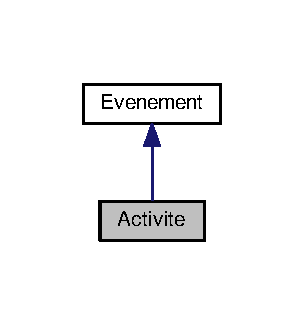
\includegraphics[width=146pt]{class_activite__inherit__graph}
\end{center}
\end{figure}


Collaboration diagram for Activite\+:\nopagebreak
\begin{figure}[H]
\begin{center}
\leavevmode
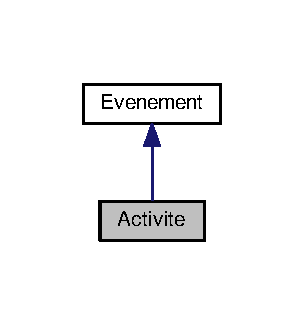
\includegraphics[width=146pt]{class_activite__coll__graph}
\end{center}
\end{figure}
\subsection*{Public Member Functions}
\begin{DoxyCompactItemize}
\item 
\hyperlink{class_activite_a06098c0f62244f4b60d250325b738094}{Activite} (const string \&t, const string \&l, \hyperlink{class_t_i_m_e_1_1_duree}{Duree} dur)
\begin{DoxyCompactList}\small\item\em Constructeur d\textquotesingle{}activité \end{DoxyCompactList}\item 
string \hyperlink{class_activite_ab0e1e83e41d35906dffc14530826075e}{get\+Titre} () const 
\begin{DoxyCompactList}\small\item\em Retourne le titre. \end{DoxyCompactList}\item 
string \hyperlink{class_activite_a695b4d43546d5715977381a7070d66d6}{get\+Lieu} () const 
\begin{DoxyCompactList}\small\item\em Retourne le lieu. \end{DoxyCompactList}\item 
void \hyperlink{class_activite_a510383c92c6d87877e074032fa8519ee}{set\+Titre} (const string \&t)
\begin{DoxyCompactList}\small\item\em Modifie le titre. \end{DoxyCompactList}\item 
void \hyperlink{class_activite_a1240cc984d5508b99feb99175bc05750}{set\+Lieu} (const string \&l)
\begin{DoxyCompactList}\small\item\em Modifie le lieu. \end{DoxyCompactList}\item 
void \hyperlink{class_activite_a513d49fbf721923d0db22a646ec606be}{update} (string t, string l, \hyperlink{class_t_i_m_e_1_1_duree}{Duree} d)
\item 
virtual void \hyperlink{class_activite_acf748b87edc5e4a5b78bd5e9364946f3}{afficher} (ostream \&f)
\begin{DoxyCompactList}\small\item\em Affiche les attributs de l\textquotesingle{}activité \end{DoxyCompactList}\end{DoxyCompactItemize}


\subsection{Detailed Description}
Classe d\textquotesingle{}evenement basique programmable, héritant d\textquotesingle{}\hyperlink{class_evenement}{Evenement} La classe possède un titre et un lieu. 

\subsection{Constructor \& Destructor Documentation}
\hypertarget{class_activite_a06098c0f62244f4b60d250325b738094}{}\index{Activite@{Activite}!Activite@{Activite}}
\index{Activite@{Activite}!Activite@{Activite}}
\subsubsection[{Activite}]{\setlength{\rightskip}{0pt plus 5cm}Activite\+::\+Activite (
\begin{DoxyParamCaption}
\item[{const string \&}]{t, }
\item[{const string \&}]{l, }
\item[{{\bf Duree}}]{dur}
\end{DoxyParamCaption}
)\hspace{0.3cm}{\ttfamily [inline]}}\label{class_activite_a06098c0f62244f4b60d250325b738094}


Constructeur d\textquotesingle{}activité 



\subsection{Member Function Documentation}
\hypertarget{class_activite_acf748b87edc5e4a5b78bd5e9364946f3}{}\index{Activite@{Activite}!afficher@{afficher}}
\index{afficher@{afficher}!Activite@{Activite}}
\subsubsection[{afficher}]{\setlength{\rightskip}{0pt plus 5cm}void Activite\+::afficher (
\begin{DoxyParamCaption}
\item[{ostream \&}]{f}
\end{DoxyParamCaption}
)\hspace{0.3cm}{\ttfamily [virtual]}}\label{class_activite_acf748b87edc5e4a5b78bd5e9364946f3}


Affiche les attributs de l\textquotesingle{}activité 



Implements \hyperlink{class_evenement_af217f0cd3d421e3f113a13536ee63593}{Evenement}.

\hypertarget{class_activite_a695b4d43546d5715977381a7070d66d6}{}\index{Activite@{Activite}!get\+Lieu@{get\+Lieu}}
\index{get\+Lieu@{get\+Lieu}!Activite@{Activite}}
\subsubsection[{get\+Lieu}]{\setlength{\rightskip}{0pt plus 5cm}string Activite\+::get\+Lieu (
\begin{DoxyParamCaption}
{}
\end{DoxyParamCaption}
) const\hspace{0.3cm}{\ttfamily [inline]}}\label{class_activite_a695b4d43546d5715977381a7070d66d6}


Retourne le lieu. 

\hypertarget{class_activite_ab0e1e83e41d35906dffc14530826075e}{}\index{Activite@{Activite}!get\+Titre@{get\+Titre}}
\index{get\+Titre@{get\+Titre}!Activite@{Activite}}
\subsubsection[{get\+Titre}]{\setlength{\rightskip}{0pt plus 5cm}string Activite\+::get\+Titre (
\begin{DoxyParamCaption}
{}
\end{DoxyParamCaption}
) const\hspace{0.3cm}{\ttfamily [inline]}}\label{class_activite_ab0e1e83e41d35906dffc14530826075e}


Retourne le titre. 

\hypertarget{class_activite_a1240cc984d5508b99feb99175bc05750}{}\index{Activite@{Activite}!set\+Lieu@{set\+Lieu}}
\index{set\+Lieu@{set\+Lieu}!Activite@{Activite}}
\subsubsection[{set\+Lieu}]{\setlength{\rightskip}{0pt plus 5cm}void Activite\+::set\+Lieu (
\begin{DoxyParamCaption}
\item[{const string \&}]{l}
\end{DoxyParamCaption}
)\hspace{0.3cm}{\ttfamily [inline]}}\label{class_activite_a1240cc984d5508b99feb99175bc05750}


Modifie le lieu. 

\hypertarget{class_activite_a510383c92c6d87877e074032fa8519ee}{}\index{Activite@{Activite}!set\+Titre@{set\+Titre}}
\index{set\+Titre@{set\+Titre}!Activite@{Activite}}
\subsubsection[{set\+Titre}]{\setlength{\rightskip}{0pt plus 5cm}void Activite\+::set\+Titre (
\begin{DoxyParamCaption}
\item[{const string \&}]{t}
\end{DoxyParamCaption}
)\hspace{0.3cm}{\ttfamily [inline]}}\label{class_activite_a510383c92c6d87877e074032fa8519ee}


Modifie le titre. 

\hypertarget{class_activite_a513d49fbf721923d0db22a646ec606be}{}\index{Activite@{Activite}!update@{update}}
\index{update@{update}!Activite@{Activite}}
\subsubsection[{update}]{\setlength{\rightskip}{0pt plus 5cm}void Activite\+::update (
\begin{DoxyParamCaption}
\item[{string}]{t, }
\item[{string}]{l, }
\item[{{\bf Duree}}]{d}
\end{DoxyParamCaption}
)\hspace{0.3cm}{\ttfamily [inline]}}\label{class_activite_a513d49fbf721923d0db22a646ec606be}
Met à jour le titre, le lieu et la durée de l\textquotesingle{}activité 

The documentation for this class was generated from the following files\+:\begin{DoxyCompactItemize}
\item 
L\+O21app/\hyperlink{_calendar_8h}{Calendar.\+h}\item 
L\+O21app/\hyperlink{_calendar_8cpp}{Calendar.\+cpp}\end{DoxyCompactItemize}

\hypertarget{class_calendar_exception}{}\section{Calendar\+Exception Class Reference}
\label{class_calendar_exception}\index{Calendar\+Exception@{Calendar\+Exception}}


Classe d\textquotesingle{}affichage des erreurs.  




{\ttfamily \#include $<$Calendar.\+h$>$}

\subsection*{Public Member Functions}
\begin{DoxyCompactItemize}
\item 
\hypertarget{class_calendar_exception_af4a976332f7659bdd866926f0145a780}{}{\bfseries Calendar\+Exception} (const string \&message)\label{class_calendar_exception_af4a976332f7659bdd866926f0145a780}

\item 
\hypertarget{class_calendar_exception_a381389e24c3efae51565bc4e7865a7d6}{}string {\bfseries get\+Info} () const \label{class_calendar_exception_a381389e24c3efae51565bc4e7865a7d6}

\end{DoxyCompactItemize}


\subsection{Detailed Description}
Classe d\textquotesingle{}affichage des erreurs. 

The documentation for this class was generated from the following file\+:\begin{DoxyCompactItemize}
\item 
L\+O21app/Calendar.\+h\end{DoxyCompactItemize}

\hypertarget{class_composite}{}\section{Composite Class Reference}
\label{class_composite}\index{Composite@{Composite}}


\hyperlink{class_tache}{Tache} qui peut contenir des tâches mais ne peut pas être programmée.  




{\ttfamily \#include $<$Calendar.\+h$>$}



Inheritance diagram for Composite\+:\nopagebreak
\begin{figure}[H]
\begin{center}
\leavevmode
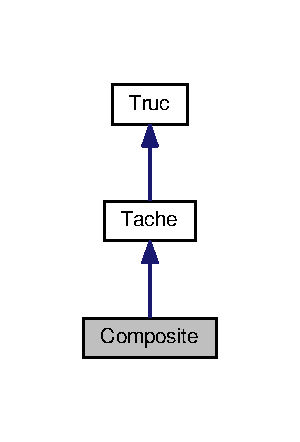
\includegraphics[width=144pt]{class_composite__inherit__graph}
\end{center}
\end{figure}


Collaboration diagram for Composite\+:\nopagebreak
\begin{figure}[H]
\begin{center}
\leavevmode
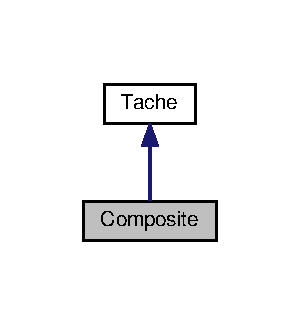
\includegraphics[width=186pt]{class_composite__coll__graph}
\end{center}
\end{figure}
\subsection*{Classes}
\begin{DoxyCompactItemize}
\item 
class \hyperlink{class_composite_1_1iterator}{iterator}
\end{DoxyCompactItemize}
\subsection*{Public Member Functions}
\begin{DoxyCompactItemize}
\item 
\hypertarget{class_composite_a63c52493ad8add53951157a418fa0971}{}\hyperlink{class_composite_1_1iterator}{iterator} {\bfseries getiterator} ()\label{class_composite_a63c52493ad8add53951157a418fa0971}

\end{DoxyCompactItemize}
\subsection*{Friends}
\begin{DoxyCompactItemize}
\item 
\hypertarget{class_composite_a67171474c4da6cc8efe0c7fafefd2b2d}{}class {\bfseries iterator}\label{class_composite_a67171474c4da6cc8efe0c7fafefd2b2d}

\end{DoxyCompactItemize}
\subsection*{Additional Inherited Members}


\subsection{Detailed Description}
\hyperlink{class_tache}{Tache} qui peut contenir des tâches mais ne peut pas être programmée. 

The documentation for this class was generated from the following file\+:\begin{DoxyCompactItemize}
\item 
L\+O21app/Calendar.\+h\end{DoxyCompactItemize}

\hypertarget{class_t_i_m_e_1_1_date}{}\section{T\+I\+M\+E\+:\+:Date Class Reference}
\label{class_t_i_m_e_1_1_date}\index{T\+I\+M\+E\+::\+Date@{T\+I\+M\+E\+::\+Date}}


Classe permettant de manipuler des dates standards L\textquotesingle{}utilisation de cette classe n�cessite des dates valides au sens commun du terme. D�clenchement d\textquotesingle{}exception dans le cas contraire.  




{\ttfamily \#include $<$timing.\+h$>$}

\subsection*{Public Member Functions}
\begin{DoxyCompactItemize}
\item 
\hyperlink{class_t_i_m_e_1_1_date_ab0d72ce6e986c0c0a5f2902e586cf81a}{Date} (unsigned int short j=1, unsigned int short m=1, unsigned int a=0)
\begin{DoxyCompactList}\small\item\em Constructeur � partir d\textquotesingle{}un jour, mois, ann�e. \end{DoxyCompactList}\item 
unsigned short int \hyperlink{class_t_i_m_e_1_1_date_a4af978b7df2b738f62449b0a7e53c21d}{get\+Jour} () const 
\begin{DoxyCompactList}\small\item\em Retourne le jour de la date. \end{DoxyCompactList}\item 
unsigned short int \hyperlink{class_t_i_m_e_1_1_date_a6cb9d945143df216115419c4cb8b14ce}{get\+Mois} () const 
\begin{DoxyCompactList}\small\item\em Retourne le mois de la date. \end{DoxyCompactList}\item 
unsigned int \hyperlink{class_t_i_m_e_1_1_date_a07b41b2e9e85ef78bf13689e772bef7d}{get\+Annee} () const 
\begin{DoxyCompactList}\small\item\em Retourne l\textquotesingle{}ann�e de la date. \end{DoxyCompactList}\item 
Q\+Date \hyperlink{class_t_i_m_e_1_1_date_a30428bf3b5e4daa144642dfa510edb14}{get\+Q\+Date} () const 
\begin{DoxyCompactList}\small\item\em Retourne l\textquotesingle{}ann�e de la date. \end{DoxyCompactList}\item 
std\+::string \hyperlink{class_t_i_m_e_1_1_date_a09b00b96742bfceaa598060b486e604c}{get\+Jour\+Mois\+String} () const 
\begin{DoxyCompactList}\small\item\em initialisation de la date \end{DoxyCompactList}\item 
void \hyperlink{class_t_i_m_e_1_1_date_a7419902750e61b9473ab05ccd5ced33d}{set\+Date} (unsigned short int j, unsigned short int m, unsigned int a)
\begin{DoxyCompactList}\small\item\em initialisation de la date avec la date d\textquotesingle{}aujourd\textquotesingle{}hui \end{DoxyCompactList}\item 
void \hyperlink{class_t_i_m_e_1_1_date_ace4be52a503c45de93b8db92dc592d93}{set\+Date\+Aujourdhui} ()
\begin{DoxyCompactList}\small\item\em affiche le date sous le format J\+J/\+M\+M/\+A\+A\+A\+A \end{DoxyCompactList}\item 
void \hyperlink{class_t_i_m_e_1_1_date_aa45188755f5d9d17cbebf0e55d3c571b}{afficher} (std\+::ostream \&f=std\+::cout) const 
\item 
bool \hyperlink{class_t_i_m_e_1_1_date_aa8208298c0efe5dbf661c66a284fd163}{operator==} (const \hyperlink{class_t_i_m_e_1_1_date}{Date} \&d) const 
\begin{DoxyCompactList}\small\item\em d1==d2 retourne vrai si les deux dates sont �gales \end{DoxyCompactList}\item 
bool \hyperlink{class_t_i_m_e_1_1_date_a8a3bccb05f00086e64c5b5518a37949f}{operator$<$} (const \hyperlink{class_t_i_m_e_1_1_date}{Date} \&d) const 
\begin{DoxyCompactList}\small\item\em Compare deux dates dans le temps \+: d1$<$d2 retourne true si d1 est avant d2. \end{DoxyCompactList}\item 
bool \hyperlink{class_t_i_m_e_1_1_date_a4e6d6c380ef57bd34506ba8f017fec67}{operator$<$=} (const \hyperlink{class_t_i_m_e_1_1_date}{Date} \&d) const 
\begin{DoxyCompactList}\small\item\em Compare deux dates dans le temps \+: d1$<$=d2 retourne true si d1 est avant ou bien �gale � d2. \end{DoxyCompactList}\item 
int \hyperlink{class_t_i_m_e_1_1_date_a61f93f8612a998bc440070f9b8a2660a}{operator-\/} (const \hyperlink{class_t_i_m_e_1_1_date}{Date} \&d) const 
\begin{DoxyCompactList}\small\item\em Retourne le nombre de jours s�parant les deux dates. \end{DoxyCompactList}\item 
\hyperlink{class_t_i_m_e_1_1_date}{Date} \hyperlink{class_t_i_m_e_1_1_date_a85907da4cadaff930c748328fda4d527}{demain} () const 
\begin{DoxyCompactList}\small\item\em Retourne la date du lendemain. \end{DoxyCompactList}\item 
\hyperlink{class_t_i_m_e_1_1_date}{Date} \hyperlink{class_t_i_m_e_1_1_date_a3c1f346c2ad9287155a71dc5d09e7fd8}{operator+} (unsigned int nb) const 
\begin{DoxyCompactList}\small\item\em Retourne la date de dans nb jours. \end{DoxyCompactList}\end{DoxyCompactItemize}
\subsection*{Static Public Member Functions}
\begin{DoxyCompactItemize}
\item 
static \hyperlink{class_t_i_m_e_1_1_date}{Date} \hyperlink{class_t_i_m_e_1_1_date_a17bb8fb342545a476f35fe745613f7a9}{to\+Timing\+Date} (Q\+Date d)
\end{DoxyCompactItemize}


\subsection{Detailed Description}
Classe permettant de manipuler des dates standards L\textquotesingle{}utilisation de cette classe n�cessite des dates valides au sens commun du terme. D�clenchement d\textquotesingle{}exception dans le cas contraire. 

\subsection{Constructor \& Destructor Documentation}
\hypertarget{class_t_i_m_e_1_1_date_ab0d72ce6e986c0c0a5f2902e586cf81a}{}\index{T\+I\+M\+E\+::\+Date@{T\+I\+M\+E\+::\+Date}!Date@{Date}}
\index{Date@{Date}!T\+I\+M\+E\+::\+Date@{T\+I\+M\+E\+::\+Date}}
\subsubsection[{Date}]{\setlength{\rightskip}{0pt plus 5cm}T\+I\+M\+E\+::\+Date\+::\+Date (
\begin{DoxyParamCaption}
\item[{unsigned int short}]{j = {\ttfamily 1}, }
\item[{unsigned int short}]{m = {\ttfamily 1}, }
\item[{unsigned int}]{a = {\ttfamily 0}}
\end{DoxyParamCaption}
)\hspace{0.3cm}{\ttfamily [inline]}}\label{class_t_i_m_e_1_1_date_ab0d72ce6e986c0c0a5f2902e586cf81a}


Constructeur � partir d\textquotesingle{}un jour, mois, ann�e. 


\begin{DoxyParams}{Parameters}
{\em j} & jour avec 1$<$=j$<$=31 \\
\hline
{\em m} & mois avec 1$<$=m$<$=12 \\
\hline
{\em a} & ann�e avec a$>$=0 \\
\hline
\end{DoxyParams}


\subsection{Member Function Documentation}
\hypertarget{class_t_i_m_e_1_1_date_aa45188755f5d9d17cbebf0e55d3c571b}{}\index{T\+I\+M\+E\+::\+Date@{T\+I\+M\+E\+::\+Date}!afficher@{afficher}}
\index{afficher@{afficher}!T\+I\+M\+E\+::\+Date@{T\+I\+M\+E\+::\+Date}}
\subsubsection[{afficher}]{\setlength{\rightskip}{0pt plus 5cm}void Date\+::afficher (
\begin{DoxyParamCaption}
\item[{std\+::ostream \&}]{f = {\ttfamily std\+:\+:cout}}
\end{DoxyParamCaption}
) const}\label{class_t_i_m_e_1_1_date_aa45188755f5d9d17cbebf0e55d3c571b}
\hypertarget{class_t_i_m_e_1_1_date_a85907da4cadaff930c748328fda4d527}{}\index{T\+I\+M\+E\+::\+Date@{T\+I\+M\+E\+::\+Date}!demain@{demain}}
\index{demain@{demain}!T\+I\+M\+E\+::\+Date@{T\+I\+M\+E\+::\+Date}}
\subsubsection[{demain}]{\setlength{\rightskip}{0pt plus 5cm}{\bf Date} Date\+::demain (
\begin{DoxyParamCaption}
{}
\end{DoxyParamCaption}
) const}\label{class_t_i_m_e_1_1_date_a85907da4cadaff930c748328fda4d527}


Retourne la date du lendemain. 

\hypertarget{class_t_i_m_e_1_1_date_a07b41b2e9e85ef78bf13689e772bef7d}{}\index{T\+I\+M\+E\+::\+Date@{T\+I\+M\+E\+::\+Date}!get\+Annee@{get\+Annee}}
\index{get\+Annee@{get\+Annee}!T\+I\+M\+E\+::\+Date@{T\+I\+M\+E\+::\+Date}}
\subsubsection[{get\+Annee}]{\setlength{\rightskip}{0pt plus 5cm}unsigned int T\+I\+M\+E\+::\+Date\+::get\+Annee (
\begin{DoxyParamCaption}
{}
\end{DoxyParamCaption}
) const\hspace{0.3cm}{\ttfamily [inline]}}\label{class_t_i_m_e_1_1_date_a07b41b2e9e85ef78bf13689e772bef7d}


Retourne l\textquotesingle{}ann�e de la date. 

\hypertarget{class_t_i_m_e_1_1_date_a4af978b7df2b738f62449b0a7e53c21d}{}\index{T\+I\+M\+E\+::\+Date@{T\+I\+M\+E\+::\+Date}!get\+Jour@{get\+Jour}}
\index{get\+Jour@{get\+Jour}!T\+I\+M\+E\+::\+Date@{T\+I\+M\+E\+::\+Date}}
\subsubsection[{get\+Jour}]{\setlength{\rightskip}{0pt plus 5cm}unsigned short int T\+I\+M\+E\+::\+Date\+::get\+Jour (
\begin{DoxyParamCaption}
{}
\end{DoxyParamCaption}
) const\hspace{0.3cm}{\ttfamily [inline]}}\label{class_t_i_m_e_1_1_date_a4af978b7df2b738f62449b0a7e53c21d}


Retourne le jour de la date. 

\hypertarget{class_t_i_m_e_1_1_date_a09b00b96742bfceaa598060b486e604c}{}\index{T\+I\+M\+E\+::\+Date@{T\+I\+M\+E\+::\+Date}!get\+Jour\+Mois\+String@{get\+Jour\+Mois\+String}}
\index{get\+Jour\+Mois\+String@{get\+Jour\+Mois\+String}!T\+I\+M\+E\+::\+Date@{T\+I\+M\+E\+::\+Date}}
\subsubsection[{get\+Jour\+Mois\+String}]{\setlength{\rightskip}{0pt plus 5cm}std\+::string T\+I\+M\+E\+::\+Date\+::get\+Jour\+Mois\+String (
\begin{DoxyParamCaption}
{}
\end{DoxyParamCaption}
) const\hspace{0.3cm}{\ttfamily [inline]}}\label{class_t_i_m_e_1_1_date_a09b00b96742bfceaa598060b486e604c}


initialisation de la date 

Retourne l\textquotesingle{}heure sous forme de chaine \hypertarget{class_t_i_m_e_1_1_date_a6cb9d945143df216115419c4cb8b14ce}{}\index{T\+I\+M\+E\+::\+Date@{T\+I\+M\+E\+::\+Date}!get\+Mois@{get\+Mois}}
\index{get\+Mois@{get\+Mois}!T\+I\+M\+E\+::\+Date@{T\+I\+M\+E\+::\+Date}}
\subsubsection[{get\+Mois}]{\setlength{\rightskip}{0pt plus 5cm}unsigned short int T\+I\+M\+E\+::\+Date\+::get\+Mois (
\begin{DoxyParamCaption}
{}
\end{DoxyParamCaption}
) const\hspace{0.3cm}{\ttfamily [inline]}}\label{class_t_i_m_e_1_1_date_a6cb9d945143df216115419c4cb8b14ce}


Retourne le mois de la date. 

\hypertarget{class_t_i_m_e_1_1_date_a30428bf3b5e4daa144642dfa510edb14}{}\index{T\+I\+M\+E\+::\+Date@{T\+I\+M\+E\+::\+Date}!get\+Q\+Date@{get\+Q\+Date}}
\index{get\+Q\+Date@{get\+Q\+Date}!T\+I\+M\+E\+::\+Date@{T\+I\+M\+E\+::\+Date}}
\subsubsection[{get\+Q\+Date}]{\setlength{\rightskip}{0pt plus 5cm}Q\+Date T\+I\+M\+E\+::\+Date\+::get\+Q\+Date (
\begin{DoxyParamCaption}
{}
\end{DoxyParamCaption}
) const\hspace{0.3cm}{\ttfamily [inline]}}\label{class_t_i_m_e_1_1_date_a30428bf3b5e4daa144642dfa510edb14}


Retourne l\textquotesingle{}ann�e de la date. 

\hypertarget{class_t_i_m_e_1_1_date_a3c1f346c2ad9287155a71dc5d09e7fd8}{}\index{T\+I\+M\+E\+::\+Date@{T\+I\+M\+E\+::\+Date}!operator+@{operator+}}
\index{operator+@{operator+}!T\+I\+M\+E\+::\+Date@{T\+I\+M\+E\+::\+Date}}
\subsubsection[{operator+}]{\setlength{\rightskip}{0pt plus 5cm}{\bf Date} Date\+::operator+ (
\begin{DoxyParamCaption}
\item[{unsigned int}]{nb}
\end{DoxyParamCaption}
) const}\label{class_t_i_m_e_1_1_date_a3c1f346c2ad9287155a71dc5d09e7fd8}


Retourne la date de dans nb jours. 

\hypertarget{class_t_i_m_e_1_1_date_a61f93f8612a998bc440070f9b8a2660a}{}\index{T\+I\+M\+E\+::\+Date@{T\+I\+M\+E\+::\+Date}!operator-\/@{operator-\/}}
\index{operator-\/@{operator-\/}!T\+I\+M\+E\+::\+Date@{T\+I\+M\+E\+::\+Date}}
\subsubsection[{operator-\/}]{\setlength{\rightskip}{0pt plus 5cm}int Date\+::operator-\/ (
\begin{DoxyParamCaption}
\item[{const {\bf Date} \&}]{d}
\end{DoxyParamCaption}
) const}\label{class_t_i_m_e_1_1_date_a61f93f8612a998bc440070f9b8a2660a}


Retourne le nombre de jours s�parant les deux dates. 

\hypertarget{class_t_i_m_e_1_1_date_a8a3bccb05f00086e64c5b5518a37949f}{}\index{T\+I\+M\+E\+::\+Date@{T\+I\+M\+E\+::\+Date}!operator$<$@{operator$<$}}
\index{operator$<$@{operator$<$}!T\+I\+M\+E\+::\+Date@{T\+I\+M\+E\+::\+Date}}
\subsubsection[{operator$<$}]{\setlength{\rightskip}{0pt plus 5cm}bool Date\+::operator$<$ (
\begin{DoxyParamCaption}
\item[{const {\bf Date} \&}]{d}
\end{DoxyParamCaption}
) const}\label{class_t_i_m_e_1_1_date_a8a3bccb05f00086e64c5b5518a37949f}


Compare deux dates dans le temps \+: d1$<$d2 retourne true si d1 est avant d2. 

\hypertarget{class_t_i_m_e_1_1_date_a4e6d6c380ef57bd34506ba8f017fec67}{}\index{T\+I\+M\+E\+::\+Date@{T\+I\+M\+E\+::\+Date}!operator$<$=@{operator$<$=}}
\index{operator$<$=@{operator$<$=}!T\+I\+M\+E\+::\+Date@{T\+I\+M\+E\+::\+Date}}
\subsubsection[{operator$<$=}]{\setlength{\rightskip}{0pt plus 5cm}bool Date\+::operator$<$= (
\begin{DoxyParamCaption}
\item[{const {\bf Date} \&}]{d}
\end{DoxyParamCaption}
) const}\label{class_t_i_m_e_1_1_date_a4e6d6c380ef57bd34506ba8f017fec67}


Compare deux dates dans le temps \+: d1$<$=d2 retourne true si d1 est avant ou bien �gale � d2. 

\hypertarget{class_t_i_m_e_1_1_date_aa8208298c0efe5dbf661c66a284fd163}{}\index{T\+I\+M\+E\+::\+Date@{T\+I\+M\+E\+::\+Date}!operator==@{operator==}}
\index{operator==@{operator==}!T\+I\+M\+E\+::\+Date@{T\+I\+M\+E\+::\+Date}}
\subsubsection[{operator==}]{\setlength{\rightskip}{0pt plus 5cm}bool Date\+::operator== (
\begin{DoxyParamCaption}
\item[{const {\bf Date} \&}]{d}
\end{DoxyParamCaption}
) const}\label{class_t_i_m_e_1_1_date_aa8208298c0efe5dbf661c66a284fd163}


d1==d2 retourne vrai si les deux dates sont �gales 

\hypertarget{class_t_i_m_e_1_1_date_a7419902750e61b9473ab05ccd5ced33d}{}\index{T\+I\+M\+E\+::\+Date@{T\+I\+M\+E\+::\+Date}!set\+Date@{set\+Date}}
\index{set\+Date@{set\+Date}!T\+I\+M\+E\+::\+Date@{T\+I\+M\+E\+::\+Date}}
\subsubsection[{set\+Date}]{\setlength{\rightskip}{0pt plus 5cm}void Date\+::set\+Date (
\begin{DoxyParamCaption}
\item[{unsigned short int}]{j, }
\item[{unsigned short int}]{m, }
\item[{unsigned int}]{a}
\end{DoxyParamCaption}
)}\label{class_t_i_m_e_1_1_date_a7419902750e61b9473ab05ccd5ced33d}


initialisation de la date avec la date d\textquotesingle{}aujourd\textquotesingle{}hui 

\hypertarget{class_t_i_m_e_1_1_date_ace4be52a503c45de93b8db92dc592d93}{}\index{T\+I\+M\+E\+::\+Date@{T\+I\+M\+E\+::\+Date}!set\+Date\+Aujourdhui@{set\+Date\+Aujourdhui}}
\index{set\+Date\+Aujourdhui@{set\+Date\+Aujourdhui}!T\+I\+M\+E\+::\+Date@{T\+I\+M\+E\+::\+Date}}
\subsubsection[{set\+Date\+Aujourdhui}]{\setlength{\rightskip}{0pt plus 5cm}void Date\+::set\+Date\+Aujourdhui (
\begin{DoxyParamCaption}
{}
\end{DoxyParamCaption}
)}\label{class_t_i_m_e_1_1_date_ace4be52a503c45de93b8db92dc592d93}


affiche le date sous le format J\+J/\+M\+M/\+A\+A\+A\+A 

\hypertarget{class_t_i_m_e_1_1_date_a17bb8fb342545a476f35fe745613f7a9}{}\index{T\+I\+M\+E\+::\+Date@{T\+I\+M\+E\+::\+Date}!to\+Timing\+Date@{to\+Timing\+Date}}
\index{to\+Timing\+Date@{to\+Timing\+Date}!T\+I\+M\+E\+::\+Date@{T\+I\+M\+E\+::\+Date}}
\subsubsection[{to\+Timing\+Date}]{\setlength{\rightskip}{0pt plus 5cm}{\bf Date} Date\+::to\+Timing\+Date (
\begin{DoxyParamCaption}
\item[{Q\+Date}]{d}
\end{DoxyParamCaption}
)\hspace{0.3cm}{\ttfamily [static]}}\label{class_t_i_m_e_1_1_date_a17bb8fb342545a476f35fe745613f7a9}


The documentation for this class was generated from the following files\+:\begin{DoxyCompactItemize}
\item 
L\+O21app/\hyperlink{timing_8h}{timing.\+h}\item 
L\+O21app/\hyperlink{timing_8cpp}{timing.\+cpp}\end{DoxyCompactItemize}

\hypertarget{class_t_i_m_e_1_1_duree}{}\section{T\+I\+M\+E\+:\+:Duree Class Reference}
\label{class_t_i_m_e_1_1_duree}\index{T\+I\+M\+E\+::\+Duree@{T\+I\+M\+E\+::\+Duree}}


Classe permettant de manipuler des durees L\textquotesingle{}utilisation de cette classe n�cessite des dates valides au sens commun du terme. D�clenchement d\textquotesingle{}exception dans le cas contraire.  




{\ttfamily \#include $<$timing.\+h$>$}

\subsection*{Public Member Functions}
\begin{DoxyCompactItemize}
\item 
\hyperlink{class_t_i_m_e_1_1_duree_ae0532a0d60dbc31773f038967dfe220e}{Duree} (unsigned int h, unsigned int m)
\begin{DoxyCompactList}\small\item\em Constructeur � partir de heure et minute. \end{DoxyCompactList}\item 
\hyperlink{class_t_i_m_e_1_1_duree_a0f99878e52fad2f9e0643301c70d9ef7}{Duree} (unsigned int m=0)
\begin{DoxyCompactList}\small\item\em Constructeur � partir de minute. \end{DoxyCompactList}\item 
void \hyperlink{class_t_i_m_e_1_1_duree_aabba3e357861f21faa8419339f7b7176}{set\+Duree} (unsigned int heures, unsigned int minutes)
\item 
unsigned int \hyperlink{class_t_i_m_e_1_1_duree_a1e47fb5f0734ec562e2f9dba32db45f4}{get\+Duree\+En\+Minutes} () const 
\begin{DoxyCompactList}\small\item\em Retourne la duree en minutes. \end{DoxyCompactList}\item 
double \hyperlink{class_t_i_m_e_1_1_duree_afb11d106fc1f6761a68f486dc7a17564}{get\+Duree\+En\+Heures} () const 
\begin{DoxyCompactList}\small\item\em Retourne la duree en heures. \end{DoxyCompactList}\item 
unsigned int \hyperlink{class_t_i_m_e_1_1_duree_aeb43e9bde7803d89edbabf040c962f9b}{get\+Duree\+En\+Heures\+Int} () const 
\begin{DoxyCompactList}\small\item\em Retourne la duree en heures tronqu�e � l\textquotesingle{}heure pr�s. \end{DoxyCompactList}\item 
void \hyperlink{class_t_i_m_e_1_1_duree_ad957a58f8bc103857f3e494bab5f60e1}{afficher} (std\+::ostream \&f=std\+::cout) const 
\begin{DoxyCompactList}\small\item\em Affiche la duree sous le format hh\+Hmm. \end{DoxyCompactList}\item 
bool \hyperlink{class_t_i_m_e_1_1_duree_a96ac8dafc768f4c52d6811a5a89cafbc}{is\+Null} ()
\end{DoxyCompactItemize}


\subsection{Detailed Description}
Classe permettant de manipuler des durees L\textquotesingle{}utilisation de cette classe n�cessite des dates valides au sens commun du terme. D�clenchement d\textquotesingle{}exception dans le cas contraire. 

\subsection{Constructor \& Destructor Documentation}
\hypertarget{class_t_i_m_e_1_1_duree_ae0532a0d60dbc31773f038967dfe220e}{}\index{T\+I\+M\+E\+::\+Duree@{T\+I\+M\+E\+::\+Duree}!Duree@{Duree}}
\index{Duree@{Duree}!T\+I\+M\+E\+::\+Duree@{T\+I\+M\+E\+::\+Duree}}
\subsubsection[{Duree}]{\setlength{\rightskip}{0pt plus 5cm}T\+I\+M\+E\+::\+Duree\+::\+Duree (
\begin{DoxyParamCaption}
\item[{unsigned int}]{h, }
\item[{unsigned int}]{m}
\end{DoxyParamCaption}
)\hspace{0.3cm}{\ttfamily [inline]}}\label{class_t_i_m_e_1_1_duree_ae0532a0d60dbc31773f038967dfe220e}


Constructeur � partir de heure et minute. 


\begin{DoxyParams}{Parameters}
{\em h} & heure avec h$>$=0 \\
\hline
{\em m} & minute avec 0$<$=m$<$=59 \\
\hline
\end{DoxyParams}
\hypertarget{class_t_i_m_e_1_1_duree_a0f99878e52fad2f9e0643301c70d9ef7}{}\index{T\+I\+M\+E\+::\+Duree@{T\+I\+M\+E\+::\+Duree}!Duree@{Duree}}
\index{Duree@{Duree}!T\+I\+M\+E\+::\+Duree@{T\+I\+M\+E\+::\+Duree}}
\subsubsection[{Duree}]{\setlength{\rightskip}{0pt plus 5cm}T\+I\+M\+E\+::\+Duree\+::\+Duree (
\begin{DoxyParamCaption}
\item[{unsigned int}]{m = {\ttfamily 0}}
\end{DoxyParamCaption}
)\hspace{0.3cm}{\ttfamily [inline]}}\label{class_t_i_m_e_1_1_duree_a0f99878e52fad2f9e0643301c70d9ef7}


Constructeur � partir de minute. 


\begin{DoxyParams}{Parameters}
{\em m} & minute avec m$>$=0 \\
\hline
\end{DoxyParams}


\subsection{Member Function Documentation}
\hypertarget{class_t_i_m_e_1_1_duree_ad957a58f8bc103857f3e494bab5f60e1}{}\index{T\+I\+M\+E\+::\+Duree@{T\+I\+M\+E\+::\+Duree}!afficher@{afficher}}
\index{afficher@{afficher}!T\+I\+M\+E\+::\+Duree@{T\+I\+M\+E\+::\+Duree}}
\subsubsection[{afficher}]{\setlength{\rightskip}{0pt plus 5cm}void T\+I\+M\+E\+::\+Duree\+::afficher (
\begin{DoxyParamCaption}
\item[{std\+::ostream \&}]{f = {\ttfamily std\+:\+:cout}}
\end{DoxyParamCaption}
) const\hspace{0.3cm}{\ttfamily [inline]}}\label{class_t_i_m_e_1_1_duree_ad957a58f8bc103857f3e494bab5f60e1}


Affiche la duree sous le format hh\+Hmm. 

\hypertarget{class_t_i_m_e_1_1_duree_afb11d106fc1f6761a68f486dc7a17564}{}\index{T\+I\+M\+E\+::\+Duree@{T\+I\+M\+E\+::\+Duree}!get\+Duree\+En\+Heures@{get\+Duree\+En\+Heures}}
\index{get\+Duree\+En\+Heures@{get\+Duree\+En\+Heures}!T\+I\+M\+E\+::\+Duree@{T\+I\+M\+E\+::\+Duree}}
\subsubsection[{get\+Duree\+En\+Heures}]{\setlength{\rightskip}{0pt plus 5cm}double T\+I\+M\+E\+::\+Duree\+::get\+Duree\+En\+Heures (
\begin{DoxyParamCaption}
{}
\end{DoxyParamCaption}
) const\hspace{0.3cm}{\ttfamily [inline]}}\label{class_t_i_m_e_1_1_duree_afb11d106fc1f6761a68f486dc7a17564}


Retourne la duree en heures. 

\hypertarget{class_t_i_m_e_1_1_duree_aeb43e9bde7803d89edbabf040c962f9b}{}\index{T\+I\+M\+E\+::\+Duree@{T\+I\+M\+E\+::\+Duree}!get\+Duree\+En\+Heures\+Int@{get\+Duree\+En\+Heures\+Int}}
\index{get\+Duree\+En\+Heures\+Int@{get\+Duree\+En\+Heures\+Int}!T\+I\+M\+E\+::\+Duree@{T\+I\+M\+E\+::\+Duree}}
\subsubsection[{get\+Duree\+En\+Heures\+Int}]{\setlength{\rightskip}{0pt plus 5cm}unsigned int T\+I\+M\+E\+::\+Duree\+::get\+Duree\+En\+Heures\+Int (
\begin{DoxyParamCaption}
{}
\end{DoxyParamCaption}
) const\hspace{0.3cm}{\ttfamily [inline]}}\label{class_t_i_m_e_1_1_duree_aeb43e9bde7803d89edbabf040c962f9b}


Retourne la duree en heures tronqu�e � l\textquotesingle{}heure pr�s. 

\hypertarget{class_t_i_m_e_1_1_duree_a1e47fb5f0734ec562e2f9dba32db45f4}{}\index{T\+I\+M\+E\+::\+Duree@{T\+I\+M\+E\+::\+Duree}!get\+Duree\+En\+Minutes@{get\+Duree\+En\+Minutes}}
\index{get\+Duree\+En\+Minutes@{get\+Duree\+En\+Minutes}!T\+I\+M\+E\+::\+Duree@{T\+I\+M\+E\+::\+Duree}}
\subsubsection[{get\+Duree\+En\+Minutes}]{\setlength{\rightskip}{0pt plus 5cm}unsigned int T\+I\+M\+E\+::\+Duree\+::get\+Duree\+En\+Minutes (
\begin{DoxyParamCaption}
{}
\end{DoxyParamCaption}
) const\hspace{0.3cm}{\ttfamily [inline]}}\label{class_t_i_m_e_1_1_duree_a1e47fb5f0734ec562e2f9dba32db45f4}


Retourne la duree en minutes. 

\hypertarget{class_t_i_m_e_1_1_duree_a96ac8dafc768f4c52d6811a5a89cafbc}{}\index{T\+I\+M\+E\+::\+Duree@{T\+I\+M\+E\+::\+Duree}!is\+Null@{is\+Null}}
\index{is\+Null@{is\+Null}!T\+I\+M\+E\+::\+Duree@{T\+I\+M\+E\+::\+Duree}}
\subsubsection[{is\+Null}]{\setlength{\rightskip}{0pt plus 5cm}bool T\+I\+M\+E\+::\+Duree\+::is\+Null (
\begin{DoxyParamCaption}
{}
\end{DoxyParamCaption}
)\hspace{0.3cm}{\ttfamily [inline]}}\label{class_t_i_m_e_1_1_duree_a96ac8dafc768f4c52d6811a5a89cafbc}
\hypertarget{class_t_i_m_e_1_1_duree_aabba3e357861f21faa8419339f7b7176}{}\index{T\+I\+M\+E\+::\+Duree@{T\+I\+M\+E\+::\+Duree}!set\+Duree@{set\+Duree}}
\index{set\+Duree@{set\+Duree}!T\+I\+M\+E\+::\+Duree@{T\+I\+M\+E\+::\+Duree}}
\subsubsection[{set\+Duree}]{\setlength{\rightskip}{0pt plus 5cm}void T\+I\+M\+E\+::\+Duree\+::set\+Duree (
\begin{DoxyParamCaption}
\item[{unsigned int}]{heures, }
\item[{unsigned int}]{minutes}
\end{DoxyParamCaption}
)\hspace{0.3cm}{\ttfamily [inline]}}\label{class_t_i_m_e_1_1_duree_aabba3e357861f21faa8419339f7b7176}


The documentation for this class was generated from the following file\+:\begin{DoxyCompactItemize}
\item 
L\+O21app/\hyperlink{timing_8h}{timing.\+h}\end{DoxyCompactItemize}

\hypertarget{class_t_i_m_e_1_1_horaire}{}\section{T\+I\+M\+E\+:\+:Horaire Class Reference}
\label{class_t_i_m_e_1_1_horaire}\index{T\+I\+M\+E\+::\+Horaire@{T\+I\+M\+E\+::\+Horaire}}


Classe permettant de manipuler des horaires L\textquotesingle{}utilisation de cette classe n�cessite des dates valides au sens commun du terme. D�clenchement d\textquotesingle{}exception dans le cas contraire.  




{\ttfamily \#include $<$timing.\+h$>$}

\subsection*{Public Member Functions}
\begin{DoxyCompactItemize}
\item 
\hyperlink{class_t_i_m_e_1_1_horaire_ab833c9dc3a4fdbda3894dbbd72643813}{Horaire} (unsigned short int h, unsigned short int m)
\begin{DoxyCompactList}\small\item\em Constructeur � partir de heure et minute. \end{DoxyCompactList}\item 
\hypertarget{class_t_i_m_e_1_1_horaire_ae4dd22490e383b0662fc5788bd42d370}{}void {\bfseries set\+Horaire} (unsigned short int h, unsigned short int m)\label{class_t_i_m_e_1_1_horaire_ae4dd22490e383b0662fc5788bd42d370}

\item 
\hypertarget{class_t_i_m_e_1_1_horaire_af4f27b26ed338d7fa03659107f813cf8}{}void {\bfseries afficher} (std\+::ostream \&f=std\+::cout) const \label{class_t_i_m_e_1_1_horaire_af4f27b26ed338d7fa03659107f813cf8}

\item 
\hypertarget{class_t_i_m_e_1_1_horaire_ace5d2381e38d80e99c6a84158a4044e3}{}unsigned short int {\bfseries get\+Heure} () const \label{class_t_i_m_e_1_1_horaire_ace5d2381e38d80e99c6a84158a4044e3}

\item 
\hypertarget{class_t_i_m_e_1_1_horaire_a5b0e73a520913fd0588407c1507344a8}{}unsigned short int {\bfseries get\+Minute} () const \label{class_t_i_m_e_1_1_horaire_a5b0e73a520913fd0588407c1507344a8}

\item 
\hypertarget{class_t_i_m_e_1_1_horaire_a30ec21c5b5cad95c1c17c02c66d796a6}{}bool {\bfseries operator$<$} (const \hyperlink{class_t_i_m_e_1_1_horaire}{Horaire} \&h) const \label{class_t_i_m_e_1_1_horaire_a30ec21c5b5cad95c1c17c02c66d796a6}

\end{DoxyCompactItemize}


\subsection{Detailed Description}
Classe permettant de manipuler des horaires L\textquotesingle{}utilisation de cette classe n�cessite des dates valides au sens commun du terme. D�clenchement d\textquotesingle{}exception dans le cas contraire. 

\subsection{Constructor \& Destructor Documentation}
\hypertarget{class_t_i_m_e_1_1_horaire_ab833c9dc3a4fdbda3894dbbd72643813}{}\index{T\+I\+M\+E\+::\+Horaire@{T\+I\+M\+E\+::\+Horaire}!Horaire@{Horaire}}
\index{Horaire@{Horaire}!T\+I\+M\+E\+::\+Horaire@{T\+I\+M\+E\+::\+Horaire}}
\subsubsection[{Horaire}]{\setlength{\rightskip}{0pt plus 5cm}T\+I\+M\+E\+::\+Horaire\+::\+Horaire (
\begin{DoxyParamCaption}
\item[{unsigned short int}]{h, }
\item[{unsigned short int}]{m}
\end{DoxyParamCaption}
)\hspace{0.3cm}{\ttfamily [inline]}}\label{class_t_i_m_e_1_1_horaire_ab833c9dc3a4fdbda3894dbbd72643813}


Constructeur � partir de heure et minute. 


\begin{DoxyParams}{Parameters}
{\em h} & heure avec 0$<$=h$<$=23 \\
\hline
{\em m} & minute avec 0$<$=m$<$=59 \\
\hline
\end{DoxyParams}


The documentation for this class was generated from the following files\+:\begin{DoxyCompactItemize}
\item 
L\+O21app/timing.\+h\item 
L\+O21app/timing.\+cpp\end{DoxyCompactItemize}

\hypertarget{class_t_i_m_e_1_1_intervalle}{}\section{T\+I\+M\+E\+:\+:Intervalle Class Reference}
\label{class_t_i_m_e_1_1_intervalle}\index{T\+I\+M\+E\+::\+Intervalle@{T\+I\+M\+E\+::\+Intervalle}}


Classe permettant de manipuler des intervalles de dates L\textquotesingle{}utilisation de cette classe n�cessite des dates valides au sens commun du terme. D�clenchement d\textquotesingle{}exception dans le cas contraire.  




{\ttfamily \#include $<$timing.\+h$>$}

\subsection*{Public Member Functions}
\begin{DoxyCompactItemize}
\item 
\hyperlink{class_t_i_m_e_1_1_intervalle_a98b63f9c55a777090ec224d61ab26427}{Intervalle} (const \hyperlink{class_t_i_m_e_1_1_date}{Date} \&d, const \hyperlink{class_t_i_m_e_1_1_date}{Date} \&f)
\begin{DoxyCompactList}\small\item\em Constructeur � partir de deux dates. \end{DoxyCompactList}\item 
void \hyperlink{class_t_i_m_e_1_1_intervalle_a729d464967de6618da00b772357dc923}{afficher} (std\+::ostream \&f=std\+::cout) const 
\begin{DoxyCompactList}\small\item\em Affiche l\textquotesingle{}intervalle de dates. \end{DoxyCompactList}\item 
\hyperlink{class_t_i_m_e_1_1_date}{Date} \hyperlink{class_t_i_m_e_1_1_intervalle_a8a9980c16e051af5e08135815cc3d074}{get\+Debut} () const 
\begin{DoxyCompactList}\small\item\em Retourne la date de d�but de l\textquotesingle{}intervalle. \end{DoxyCompactList}\item 
\hyperlink{class_t_i_m_e_1_1_date}{Date} \hyperlink{class_t_i_m_e_1_1_intervalle_a20a035fb9d9720ef94e62e1ef45845c3}{get\+Fin} () const 
\begin{DoxyCompactList}\small\item\em Retourne la date de fin de l\textquotesingle{}intervalle. \end{DoxyCompactList}\item 
int \hyperlink{class_t_i_m_e_1_1_intervalle_adec63857259b690f79de8d16b0ca0c4d}{get\+Duree} () const 
\begin{DoxyCompactList}\small\item\em Retourne le nombre de jours s\textquotesingle{}�coulant entre le d�but et la fin de l\textquotesingle{}intervalle. \end{DoxyCompactList}\item 
bool \hyperlink{class_t_i_m_e_1_1_intervalle_a8f7dca71eb9d8648fa30225360df4fda}{operator\&\&} (const \hyperlink{class_t_i_m_e_1_1_intervalle}{Intervalle} \&v) const 
\begin{DoxyCompactList}\small\item\em I1\&\&I2 Retourne vrai si il y a intersection entre I1 et I2. \end{DoxyCompactList}\item 
\hyperlink{class_t_i_m_e_1_1_intervalle}{Intervalle} \hyperlink{class_t_i_m_e_1_1_intervalle_a9dfead5501b190507a2ffa5c29450ffe}{operator+} (const \hyperlink{class_t_i_m_e_1_1_intervalle}{Intervalle} \&i) const 
\begin{DoxyCompactList}\small\item\em I1+\+I2 Retourne un intervalle union des 2 intervalles I1 et I2 qui se touchent, ie I2.\+debut est le jour du lendemain de I1.\+fin. \end{DoxyCompactList}\end{DoxyCompactItemize}


\subsection{Detailed Description}
Classe permettant de manipuler des intervalles de dates L\textquotesingle{}utilisation de cette classe n�cessite des dates valides au sens commun du terme. D�clenchement d\textquotesingle{}exception dans le cas contraire. 

\subsection{Constructor \& Destructor Documentation}
\hypertarget{class_t_i_m_e_1_1_intervalle_a98b63f9c55a777090ec224d61ab26427}{}\index{T\+I\+M\+E\+::\+Intervalle@{T\+I\+M\+E\+::\+Intervalle}!Intervalle@{Intervalle}}
\index{Intervalle@{Intervalle}!T\+I\+M\+E\+::\+Intervalle@{T\+I\+M\+E\+::\+Intervalle}}
\subsubsection[{Intervalle}]{\setlength{\rightskip}{0pt plus 5cm}Intervalle\+::\+Intervalle (
\begin{DoxyParamCaption}
\item[{const {\bf Date} \&}]{d, }
\item[{const {\bf Date} \&}]{f}
\end{DoxyParamCaption}
)}\label{class_t_i_m_e_1_1_intervalle_a98b63f9c55a777090ec224d61ab26427}


Constructeur � partir de deux dates. 


\begin{DoxyParams}{Parameters}
{\em d} & date de d�but de l\textquotesingle{}intervalle \\
\hline
{\em f} & date de fin de l\textquotesingle{}intervalle. On doit avoir d$<$=f \\
\hline
\end{DoxyParams}


\subsection{Member Function Documentation}
\hypertarget{class_t_i_m_e_1_1_intervalle_a729d464967de6618da00b772357dc923}{}\index{T\+I\+M\+E\+::\+Intervalle@{T\+I\+M\+E\+::\+Intervalle}!afficher@{afficher}}
\index{afficher@{afficher}!T\+I\+M\+E\+::\+Intervalle@{T\+I\+M\+E\+::\+Intervalle}}
\subsubsection[{afficher}]{\setlength{\rightskip}{0pt plus 5cm}void Intervalle\+::afficher (
\begin{DoxyParamCaption}
\item[{std\+::ostream \&}]{f = {\ttfamily std\+:\+:cout}}
\end{DoxyParamCaption}
) const}\label{class_t_i_m_e_1_1_intervalle_a729d464967de6618da00b772357dc923}


Affiche l\textquotesingle{}intervalle de dates. 

\hypertarget{class_t_i_m_e_1_1_intervalle_a8a9980c16e051af5e08135815cc3d074}{}\index{T\+I\+M\+E\+::\+Intervalle@{T\+I\+M\+E\+::\+Intervalle}!get\+Debut@{get\+Debut}}
\index{get\+Debut@{get\+Debut}!T\+I\+M\+E\+::\+Intervalle@{T\+I\+M\+E\+::\+Intervalle}}
\subsubsection[{get\+Debut}]{\setlength{\rightskip}{0pt plus 5cm}{\bf Date} T\+I\+M\+E\+::\+Intervalle\+::get\+Debut (
\begin{DoxyParamCaption}
{}
\end{DoxyParamCaption}
) const\hspace{0.3cm}{\ttfamily [inline]}}\label{class_t_i_m_e_1_1_intervalle_a8a9980c16e051af5e08135815cc3d074}


Retourne la date de d�but de l\textquotesingle{}intervalle. 

\hypertarget{class_t_i_m_e_1_1_intervalle_adec63857259b690f79de8d16b0ca0c4d}{}\index{T\+I\+M\+E\+::\+Intervalle@{T\+I\+M\+E\+::\+Intervalle}!get\+Duree@{get\+Duree}}
\index{get\+Duree@{get\+Duree}!T\+I\+M\+E\+::\+Intervalle@{T\+I\+M\+E\+::\+Intervalle}}
\subsubsection[{get\+Duree}]{\setlength{\rightskip}{0pt plus 5cm}int T\+I\+M\+E\+::\+Intervalle\+::get\+Duree (
\begin{DoxyParamCaption}
{}
\end{DoxyParamCaption}
) const\hspace{0.3cm}{\ttfamily [inline]}}\label{class_t_i_m_e_1_1_intervalle_adec63857259b690f79de8d16b0ca0c4d}


Retourne le nombre de jours s\textquotesingle{}�coulant entre le d�but et la fin de l\textquotesingle{}intervalle. 

\hypertarget{class_t_i_m_e_1_1_intervalle_a20a035fb9d9720ef94e62e1ef45845c3}{}\index{T\+I\+M\+E\+::\+Intervalle@{T\+I\+M\+E\+::\+Intervalle}!get\+Fin@{get\+Fin}}
\index{get\+Fin@{get\+Fin}!T\+I\+M\+E\+::\+Intervalle@{T\+I\+M\+E\+::\+Intervalle}}
\subsubsection[{get\+Fin}]{\setlength{\rightskip}{0pt plus 5cm}{\bf Date} T\+I\+M\+E\+::\+Intervalle\+::get\+Fin (
\begin{DoxyParamCaption}
{}
\end{DoxyParamCaption}
) const\hspace{0.3cm}{\ttfamily [inline]}}\label{class_t_i_m_e_1_1_intervalle_a20a035fb9d9720ef94e62e1ef45845c3}


Retourne la date de fin de l\textquotesingle{}intervalle. 

\hypertarget{class_t_i_m_e_1_1_intervalle_a8f7dca71eb9d8648fa30225360df4fda}{}\index{T\+I\+M\+E\+::\+Intervalle@{T\+I\+M\+E\+::\+Intervalle}!operator\&\&@{operator\&\&}}
\index{operator\&\&@{operator\&\&}!T\+I\+M\+E\+::\+Intervalle@{T\+I\+M\+E\+::\+Intervalle}}
\subsubsection[{operator\&\&}]{\setlength{\rightskip}{0pt plus 5cm}bool Intervalle\+::operator\&\& (
\begin{DoxyParamCaption}
\item[{const {\bf Intervalle} \&}]{v}
\end{DoxyParamCaption}
) const}\label{class_t_i_m_e_1_1_intervalle_a8f7dca71eb9d8648fa30225360df4fda}


I1\&\&I2 Retourne vrai si il y a intersection entre I1 et I2. 

\hypertarget{class_t_i_m_e_1_1_intervalle_a9dfead5501b190507a2ffa5c29450ffe}{}\index{T\+I\+M\+E\+::\+Intervalle@{T\+I\+M\+E\+::\+Intervalle}!operator+@{operator+}}
\index{operator+@{operator+}!T\+I\+M\+E\+::\+Intervalle@{T\+I\+M\+E\+::\+Intervalle}}
\subsubsection[{operator+}]{\setlength{\rightskip}{0pt plus 5cm}{\bf Intervalle} Intervalle\+::operator+ (
\begin{DoxyParamCaption}
\item[{const {\bf Intervalle} \&}]{i}
\end{DoxyParamCaption}
) const}\label{class_t_i_m_e_1_1_intervalle_a9dfead5501b190507a2ffa5c29450ffe}


I1+\+I2 Retourne un intervalle union des 2 intervalles I1 et I2 qui se touchent, ie I2.\+debut est le jour du lendemain de I1.\+fin. 



The documentation for this class was generated from the following files\+:\begin{DoxyCompactItemize}
\item 
L\+O21app/\hyperlink{timing_8h}{timing.\+h}\item 
L\+O21app/\hyperlink{timing_8cpp}{timing.\+cpp}\end{DoxyCompactItemize}

\hypertarget{class_tache_1_1_iterator}{}\section{Tache\+:\+:Iterator Class Reference}
\label{class_tache_1_1_iterator}\index{Tache\+::\+Iterator@{Tache\+::\+Iterator}}


{\ttfamily \#include $<$Calendar.\+h$>$}

\subsection*{Public Member Functions}
\begin{DoxyCompactItemize}
\item 
\hyperlink{class_tache}{Tache} \& \hyperlink{class_tache_1_1_iterator_a14d6234f2a8ea2c4e87687375272123a}{current} () const 
\item 
bool \hyperlink{class_tache_1_1_iterator_a8130c3fa6c6cd3c9e2489162e3a01e56}{is\+Done} () const 
\item 
void \hyperlink{class_tache_1_1_iterator_ae9d3e979ec79eb49a73be93391d171a0}{next} ()
\item 
void \hyperlink{class_tache_1_1_iterator_a7329120b9efd311ef5ab48a42c997be8}{first} ()
\end{DoxyCompactItemize}
\subsection*{Friends}
\begin{DoxyCompactItemize}
\item 
class \hyperlink{class_tache_1_1_iterator_affcde2942f74e98f2e6e352cba2a1dc1}{Tache}
\end{DoxyCompactItemize}


\subsection{Member Function Documentation}
\hypertarget{class_tache_1_1_iterator_a14d6234f2a8ea2c4e87687375272123a}{}\index{Tache\+::\+Iterator@{Tache\+::\+Iterator}!current@{current}}
\index{current@{current}!Tache\+::\+Iterator@{Tache\+::\+Iterator}}
\subsubsection[{current}]{\setlength{\rightskip}{0pt plus 5cm}{\bf Tache}\& Tache\+::\+Iterator\+::current (
\begin{DoxyParamCaption}
{}
\end{DoxyParamCaption}
) const\hspace{0.3cm}{\ttfamily [inline]}}\label{class_tache_1_1_iterator_a14d6234f2a8ea2c4e87687375272123a}
\hypertarget{class_tache_1_1_iterator_a7329120b9efd311ef5ab48a42c997be8}{}\index{Tache\+::\+Iterator@{Tache\+::\+Iterator}!first@{first}}
\index{first@{first}!Tache\+::\+Iterator@{Tache\+::\+Iterator}}
\subsubsection[{first}]{\setlength{\rightskip}{0pt plus 5cm}void Tache\+::\+Iterator\+::first (
\begin{DoxyParamCaption}
{}
\end{DoxyParamCaption}
)\hspace{0.3cm}{\ttfamily [inline]}}\label{class_tache_1_1_iterator_a7329120b9efd311ef5ab48a42c997be8}
\hypertarget{class_tache_1_1_iterator_a8130c3fa6c6cd3c9e2489162e3a01e56}{}\index{Tache\+::\+Iterator@{Tache\+::\+Iterator}!is\+Done@{is\+Done}}
\index{is\+Done@{is\+Done}!Tache\+::\+Iterator@{Tache\+::\+Iterator}}
\subsubsection[{is\+Done}]{\setlength{\rightskip}{0pt plus 5cm}bool Tache\+::\+Iterator\+::is\+Done (
\begin{DoxyParamCaption}
{}
\end{DoxyParamCaption}
) const\hspace{0.3cm}{\ttfamily [inline]}}\label{class_tache_1_1_iterator_a8130c3fa6c6cd3c9e2489162e3a01e56}
\hypertarget{class_tache_1_1_iterator_ae9d3e979ec79eb49a73be93391d171a0}{}\index{Tache\+::\+Iterator@{Tache\+::\+Iterator}!next@{next}}
\index{next@{next}!Tache\+::\+Iterator@{Tache\+::\+Iterator}}
\subsubsection[{next}]{\setlength{\rightskip}{0pt plus 5cm}void Tache\+::\+Iterator\+::next (
\begin{DoxyParamCaption}
{}
\end{DoxyParamCaption}
)\hspace{0.3cm}{\ttfamily [inline]}}\label{class_tache_1_1_iterator_ae9d3e979ec79eb49a73be93391d171a0}


\subsection{Friends And Related Function Documentation}
\hypertarget{class_tache_1_1_iterator_affcde2942f74e98f2e6e352cba2a1dc1}{}\index{Tache\+::\+Iterator@{Tache\+::\+Iterator}!Tache@{Tache}}
\index{Tache@{Tache}!Tache\+::\+Iterator@{Tache\+::\+Iterator}}
\subsubsection[{Tache}]{\setlength{\rightskip}{0pt plus 5cm}friend class {\bf Tache}\hspace{0.3cm}{\ttfamily [friend]}}\label{class_tache_1_1_iterator_affcde2942f74e98f2e6e352cba2a1dc1}


The documentation for this class was generated from the following file\+:\begin{DoxyCompactItemize}
\item 
L\+O21app/\hyperlink{_calendar_8h}{Calendar.\+h}\end{DoxyCompactItemize}

\hypertarget{class_projet_1_1_iterator}{}\section{Projet\+:\+:Iterator Class Reference}
\label{class_projet_1_1_iterator}\index{Projet\+::\+Iterator@{Projet\+::\+Iterator}}


{\ttfamily \#include $<$Calendar.\+h$>$}

\subsection*{Public Member Functions}
\begin{DoxyCompactItemize}
\item 
\hyperlink{class_tache}{Tache} \& \hyperlink{class_projet_1_1_iterator_ad86c65c6828ffdce66bd5d77851acf72}{current} () const 
\item 
bool \hyperlink{class_projet_1_1_iterator_ab1cb3afe4732de443b1a4987a3888675}{is\+Done} () const 
\item 
void \hyperlink{class_projet_1_1_iterator_a2e93894b4d3ec6961fa227f52d720b19}{next} ()
\item 
void \hyperlink{class_projet_1_1_iterator_a2c2d2e1c2a601d6123048efa0d48daf6}{first} ()
\item 
void \hyperlink{class_projet_1_1_iterator_ada239ae15cfc62097e0461034f1be1d7}{suppr} ()
\end{DoxyCompactItemize}
\subsection*{Friends}
\begin{DoxyCompactItemize}
\item 
class \hyperlink{class_projet_1_1_iterator_ab87b41c3faa36955cc370972f5cce344}{Projet}
\end{DoxyCompactItemize}


\subsection{Member Function Documentation}
\hypertarget{class_projet_1_1_iterator_ad86c65c6828ffdce66bd5d77851acf72}{}\index{Projet\+::\+Iterator@{Projet\+::\+Iterator}!current@{current}}
\index{current@{current}!Projet\+::\+Iterator@{Projet\+::\+Iterator}}
\subsubsection[{current}]{\setlength{\rightskip}{0pt plus 5cm}{\bf Tache}\& Projet\+::\+Iterator\+::current (
\begin{DoxyParamCaption}
{}
\end{DoxyParamCaption}
) const\hspace{0.3cm}{\ttfamily [inline]}}\label{class_projet_1_1_iterator_ad86c65c6828ffdce66bd5d77851acf72}
\hypertarget{class_projet_1_1_iterator_a2c2d2e1c2a601d6123048efa0d48daf6}{}\index{Projet\+::\+Iterator@{Projet\+::\+Iterator}!first@{first}}
\index{first@{first}!Projet\+::\+Iterator@{Projet\+::\+Iterator}}
\subsubsection[{first}]{\setlength{\rightskip}{0pt plus 5cm}void Projet\+::\+Iterator\+::first (
\begin{DoxyParamCaption}
{}
\end{DoxyParamCaption}
)\hspace{0.3cm}{\ttfamily [inline]}}\label{class_projet_1_1_iterator_a2c2d2e1c2a601d6123048efa0d48daf6}
\hypertarget{class_projet_1_1_iterator_ab1cb3afe4732de443b1a4987a3888675}{}\index{Projet\+::\+Iterator@{Projet\+::\+Iterator}!is\+Done@{is\+Done}}
\index{is\+Done@{is\+Done}!Projet\+::\+Iterator@{Projet\+::\+Iterator}}
\subsubsection[{is\+Done}]{\setlength{\rightskip}{0pt plus 5cm}bool Projet\+::\+Iterator\+::is\+Done (
\begin{DoxyParamCaption}
{}
\end{DoxyParamCaption}
) const\hspace{0.3cm}{\ttfamily [inline]}}\label{class_projet_1_1_iterator_ab1cb3afe4732de443b1a4987a3888675}
\hypertarget{class_projet_1_1_iterator_a2e93894b4d3ec6961fa227f52d720b19}{}\index{Projet\+::\+Iterator@{Projet\+::\+Iterator}!next@{next}}
\index{next@{next}!Projet\+::\+Iterator@{Projet\+::\+Iterator}}
\subsubsection[{next}]{\setlength{\rightskip}{0pt plus 5cm}void Projet\+::\+Iterator\+::next (
\begin{DoxyParamCaption}
{}
\end{DoxyParamCaption}
)\hspace{0.3cm}{\ttfamily [inline]}}\label{class_projet_1_1_iterator_a2e93894b4d3ec6961fa227f52d720b19}
\hypertarget{class_projet_1_1_iterator_ada239ae15cfc62097e0461034f1be1d7}{}\index{Projet\+::\+Iterator@{Projet\+::\+Iterator}!suppr@{suppr}}
\index{suppr@{suppr}!Projet\+::\+Iterator@{Projet\+::\+Iterator}}
\subsubsection[{suppr}]{\setlength{\rightskip}{0pt plus 5cm}void Projet\+::\+Iterator\+::suppr (
\begin{DoxyParamCaption}
{}
\end{DoxyParamCaption}
)}\label{class_projet_1_1_iterator_ada239ae15cfc62097e0461034f1be1d7}


\subsection{Friends And Related Function Documentation}
\hypertarget{class_projet_1_1_iterator_ab87b41c3faa36955cc370972f5cce344}{}\index{Projet\+::\+Iterator@{Projet\+::\+Iterator}!Projet@{Projet}}
\index{Projet@{Projet}!Projet\+::\+Iterator@{Projet\+::\+Iterator}}
\subsubsection[{Projet}]{\setlength{\rightskip}{0pt plus 5cm}friend class {\bf Projet}\hspace{0.3cm}{\ttfamily [friend]}}\label{class_projet_1_1_iterator_ab87b41c3faa36955cc370972f5cce344}


The documentation for this class was generated from the following files\+:\begin{DoxyCompactItemize}
\item 
L\+O21app/\hyperlink{_calendar_8h}{Calendar.\+h}\item 
L\+O21app/\hyperlink{_calendar_8cpp}{Calendar.\+cpp}\end{DoxyCompactItemize}

\hypertarget{class_composite_1_1iterator}{}\section{Composite\+:\+:iterator Class Reference}
\label{class_composite_1_1iterator}\index{Composite\+::iterator@{Composite\+::iterator}}
\subsection*{Public Member Functions}
\begin{DoxyCompactItemize}
\item 
\hypertarget{class_composite_1_1iterator_aa5b6cb21a09480750f9a4d6f58c1d113}{}\hyperlink{class_tache}{Tache} \& {\bfseries current} () const \label{class_composite_1_1iterator_aa5b6cb21a09480750f9a4d6f58c1d113}

\item 
\hypertarget{class_composite_1_1iterator_a6e63e8c910e09fd8944bc29f6de15aa1}{}bool {\bfseries is\+Done} () const \label{class_composite_1_1iterator_a6e63e8c910e09fd8944bc29f6de15aa1}

\item 
\hypertarget{class_composite_1_1iterator_a6e4cc2fa35408408fa6dbd95507bb1b4}{}void {\bfseries next} ()\label{class_composite_1_1iterator_a6e4cc2fa35408408fa6dbd95507bb1b4}

\item 
\hypertarget{class_composite_1_1iterator_a222c5f6fe4e2dcc25e39700d3d50daae}{}void {\bfseries first} ()\label{class_composite_1_1iterator_a222c5f6fe4e2dcc25e39700d3d50daae}

\end{DoxyCompactItemize}
\subsection*{Friends}
\begin{DoxyCompactItemize}
\item 
\hypertarget{class_composite_1_1iterator_ace19a20e83d0e04d1929284108a7582d}{}class {\bfseries Composite}\label{class_composite_1_1iterator_ace19a20e83d0e04d1929284108a7582d}

\end{DoxyCompactItemize}


The documentation for this class was generated from the following file\+:\begin{DoxyCompactItemize}
\item 
L\+O21app/Calendar.\+h\end{DoxyCompactItemize}

\hypertarget{class_main_window}{}\section{Main\+Window Class Reference}
\label{class_main_window}\index{Main\+Window@{Main\+Window}}


Conserve les pointeurs vers les principaux widgets de la fenêtre. S\textquotesingle{}occupe des actions générales sur ceux-\/ci.  




{\ttfamily \#include $<$Main\+Window.\+h$>$}



Inheritance diagram for Main\+Window\+:\nopagebreak
\begin{figure}[H]
\begin{center}
\leavevmode
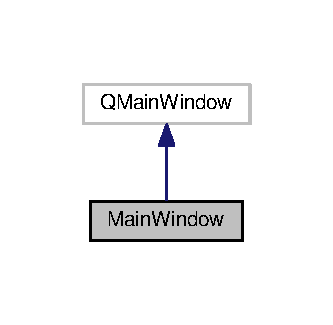
\includegraphics[width=160pt]{class_main_window__inherit__graph}
\end{center}
\end{figure}


Collaboration diagram for Main\+Window\+:\nopagebreak
\begin{figure}[H]
\begin{center}
\leavevmode
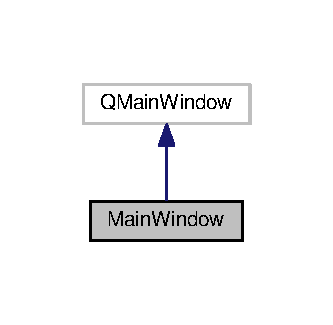
\includegraphics[width=160pt]{class_main_window__coll__graph}
\end{center}
\end{figure}
\subsection*{Public Slots}
\begin{DoxyCompactItemize}
\item 
void \hyperlink{class_main_window_a4e6f43d07f77bfa5ef816fdaeddb2f9c}{tree\+View\+Clicked} (const Q\+Model\+Index \&index)
\begin{DoxyCompactList}\small\item\em On traite le clic sur l\textquotesingle{}item index de la vue Tree\+View. \end{DoxyCompactList}\item 
void \hyperlink{class_main_window_a9221bf94c502faa7f0cb55835dc4f576}{slot\+Ajouter\+Projet} ()
\begin{DoxyCompactList}\small\item\em Ajoute un projet dans le système et sur l\textquotesingle{}arbre. \end{DoxyCompactList}\item 
void \hyperlink{class_main_window_addf6fb45b7869279d5c7b746dfe61429}{slot\+Ajouter\+T\+U} ()
\begin{DoxyCompactList}\small\item\em Ajoute une tache unitaire dans le système et sur l\textquotesingle{}arbre. \end{DoxyCompactList}\item 
void \hyperlink{class_main_window_a4201a4ae86be39f54071eedb95af8291}{slot\+Ajouter\+T\+C} ()
\begin{DoxyCompactList}\small\item\em Ajoute une tache composite dans le système et sur l\textquotesingle{}arbre. \end{DoxyCompactList}\item 
void \hyperlink{class_main_window_a2022b216fafd6461b8b959e791fee853}{slot\+Show\+T\+U} ()
\begin{DoxyCompactList}\small\item\em Lance l\textquotesingle{}affichage de l\textquotesingle{}édition de la tache t. \end{DoxyCompactList}\item 
void \hyperlink{class_main_window_a72cb9533595d3347763e3e485ac01fd6}{slot\+Show\+T\+C} ()
\begin{DoxyCompactList}\small\item\em Lance l\textquotesingle{}affichage de l\textquotesingle{}édition de la tache t. \end{DoxyCompactList}\item 
void \hyperlink{class_main_window_a22bdfd5758d79d8a0dd6b55817f053a0}{slot\+Programmer\+T\+U} ()
\begin{DoxyCompactList}\small\item\em Lance le dialogue pour programmer une tache unitaire. \end{DoxyCompactList}\item 
void \hyperlink{class_main_window_ac54011d65e21b9a451a255c8ab2856d0}{slot\+Programmer\+Activite} ()
\begin{DoxyCompactList}\small\item\em Lance le dialogue pour programmer une activité \end{DoxyCompactList}\end{DoxyCompactItemize}
\subsection*{Public Member Functions}
\begin{DoxyCompactItemize}
\item 
\hyperlink{class_main_window_ae98d00a93bc118200eeef9f9bba1dba7}{$\sim$\+Main\+Window} ()
\item 
\hyperlink{class_main_window_a34c4b4207b46d11a4100c9b19f0e81bb}{Main\+Window} ()
\begin{DoxyCompactList}\small\item\em initialisation de la fenêtre principale \end{DoxyCompactList}\item 
void \hyperlink{class_main_window_a7bbdf27e0ee846803813e53a39a3bf01}{show\+Unitaire} (\hyperlink{class_unitaire}{Unitaire} \&t)
\begin{DoxyCompactList}\small\item\em Affiche l\textquotesingle{}édition d\textquotesingle{}une tache unitaire. \end{DoxyCompactList}\item 
void \hyperlink{class_main_window_a4d74b656f89425afefef0505508befe7}{save\+Unitaire} ()
\begin{DoxyCompactList}\small\item\em Enregistre une tache unitaire. \end{DoxyCompactList}\item 
void \hyperlink{class_main_window_aad741802f157d624081f9588a120f016}{show\+Composite} (\hyperlink{class_composite}{Composite} \&t)
\begin{DoxyCompactList}\small\item\em Affiche l\textquotesingle{}édition d\textquotesingle{} tache composite. \end{DoxyCompactList}\item 
void \hyperlink{class_main_window_a1dfed2a765d3fa7bfb340dd37a5350f1}{show\+Projet} (\hyperlink{class_projet}{Projet} \&p)
\begin{DoxyCompactList}\small\item\em Affiche l\textquotesingle{}édition d\textquotesingle{}un projet. \end{DoxyCompactList}\end{DoxyCompactItemize}


\subsection{Detailed Description}
Conserve les pointeurs vers les principaux widgets de la fenêtre. S\textquotesingle{}occupe des actions générales sur ceux-\/ci. 

Cette classe fait appel aux fonctions d\textquotesingle{}affichage de \hyperlink{_u_i_classes_8h}{U\+I\+Classes.\+h} 

\subsection{Constructor \& Destructor Documentation}
\hypertarget{class_main_window_ae98d00a93bc118200eeef9f9bba1dba7}{}\index{Main\+Window@{Main\+Window}!````~Main\+Window@{$\sim$\+Main\+Window}}
\index{````~Main\+Window@{$\sim$\+Main\+Window}!Main\+Window@{Main\+Window}}
\subsubsection[{$\sim$\+Main\+Window}]{\setlength{\rightskip}{0pt plus 5cm}Main\+Window\+::$\sim$\+Main\+Window (
\begin{DoxyParamCaption}
{}
\end{DoxyParamCaption}
)\hspace{0.3cm}{\ttfamily [inline]}}\label{class_main_window_ae98d00a93bc118200eeef9f9bba1dba7}
\hypertarget{class_main_window_a34c4b4207b46d11a4100c9b19f0e81bb}{}\index{Main\+Window@{Main\+Window}!Main\+Window@{Main\+Window}}
\index{Main\+Window@{Main\+Window}!Main\+Window@{Main\+Window}}
\subsubsection[{Main\+Window}]{\setlength{\rightskip}{0pt plus 5cm}Main\+Window\+::\+Main\+Window (
\begin{DoxyParamCaption}
{}
\end{DoxyParamCaption}
)}\label{class_main_window_a34c4b4207b46d11a4100c9b19f0e81bb}


initialisation de la fenêtre principale 



\subsection{Member Function Documentation}
\hypertarget{class_main_window_a4d74b656f89425afefef0505508befe7}{}\index{Main\+Window@{Main\+Window}!save\+Unitaire@{save\+Unitaire}}
\index{save\+Unitaire@{save\+Unitaire}!Main\+Window@{Main\+Window}}
\subsubsection[{save\+Unitaire}]{\setlength{\rightskip}{0pt plus 5cm}void Main\+Window\+::save\+Unitaire (
\begin{DoxyParamCaption}
{}
\end{DoxyParamCaption}
)}\label{class_main_window_a4d74b656f89425afefef0505508befe7}


Enregistre une tache unitaire. 

\hypertarget{class_main_window_aad741802f157d624081f9588a120f016}{}\index{Main\+Window@{Main\+Window}!show\+Composite@{show\+Composite}}
\index{show\+Composite@{show\+Composite}!Main\+Window@{Main\+Window}}
\subsubsection[{show\+Composite}]{\setlength{\rightskip}{0pt plus 5cm}void Main\+Window\+::show\+Composite (
\begin{DoxyParamCaption}
\item[{{\bf Composite} \&}]{t}
\end{DoxyParamCaption}
)}\label{class_main_window_aad741802f157d624081f9588a120f016}


Affiche l\textquotesingle{}édition d\textquotesingle{} tache composite. 

\hypertarget{class_main_window_a1dfed2a765d3fa7bfb340dd37a5350f1}{}\index{Main\+Window@{Main\+Window}!show\+Projet@{show\+Projet}}
\index{show\+Projet@{show\+Projet}!Main\+Window@{Main\+Window}}
\subsubsection[{show\+Projet}]{\setlength{\rightskip}{0pt plus 5cm}void Main\+Window\+::show\+Projet (
\begin{DoxyParamCaption}
\item[{{\bf Projet} \&}]{p}
\end{DoxyParamCaption}
)}\label{class_main_window_a1dfed2a765d3fa7bfb340dd37a5350f1}


Affiche l\textquotesingle{}édition d\textquotesingle{}un projet. 

\hypertarget{class_main_window_a7bbdf27e0ee846803813e53a39a3bf01}{}\index{Main\+Window@{Main\+Window}!show\+Unitaire@{show\+Unitaire}}
\index{show\+Unitaire@{show\+Unitaire}!Main\+Window@{Main\+Window}}
\subsubsection[{show\+Unitaire}]{\setlength{\rightskip}{0pt plus 5cm}void Main\+Window\+::show\+Unitaire (
\begin{DoxyParamCaption}
\item[{{\bf Unitaire} \&}]{t}
\end{DoxyParamCaption}
)}\label{class_main_window_a7bbdf27e0ee846803813e53a39a3bf01}


Affiche l\textquotesingle{}édition d\textquotesingle{}une tache unitaire. 

\hypertarget{class_main_window_a9221bf94c502faa7f0cb55835dc4f576}{}\index{Main\+Window@{Main\+Window}!slot\+Ajouter\+Projet@{slot\+Ajouter\+Projet}}
\index{slot\+Ajouter\+Projet@{slot\+Ajouter\+Projet}!Main\+Window@{Main\+Window}}
\subsubsection[{slot\+Ajouter\+Projet}]{\setlength{\rightskip}{0pt plus 5cm}void Main\+Window\+::slot\+Ajouter\+Projet (
\begin{DoxyParamCaption}
{}
\end{DoxyParamCaption}
)\hspace{0.3cm}{\ttfamily [slot]}}\label{class_main_window_a9221bf94c502faa7f0cb55835dc4f576}


Ajoute un projet dans le système et sur l\textquotesingle{}arbre. 

\hypertarget{class_main_window_a4201a4ae86be39f54071eedb95af8291}{}\index{Main\+Window@{Main\+Window}!slot\+Ajouter\+T\+C@{slot\+Ajouter\+T\+C}}
\index{slot\+Ajouter\+T\+C@{slot\+Ajouter\+T\+C}!Main\+Window@{Main\+Window}}
\subsubsection[{slot\+Ajouter\+T\+C}]{\setlength{\rightskip}{0pt plus 5cm}void Main\+Window\+::slot\+Ajouter\+T\+C (
\begin{DoxyParamCaption}
{}
\end{DoxyParamCaption}
)\hspace{0.3cm}{\ttfamily [slot]}}\label{class_main_window_a4201a4ae86be39f54071eedb95af8291}


Ajoute une tache composite dans le système et sur l\textquotesingle{}arbre. 

\hypertarget{class_main_window_addf6fb45b7869279d5c7b746dfe61429}{}\index{Main\+Window@{Main\+Window}!slot\+Ajouter\+T\+U@{slot\+Ajouter\+T\+U}}
\index{slot\+Ajouter\+T\+U@{slot\+Ajouter\+T\+U}!Main\+Window@{Main\+Window}}
\subsubsection[{slot\+Ajouter\+T\+U}]{\setlength{\rightskip}{0pt plus 5cm}void Main\+Window\+::slot\+Ajouter\+T\+U (
\begin{DoxyParamCaption}
{}
\end{DoxyParamCaption}
)\hspace{0.3cm}{\ttfamily [slot]}}\label{class_main_window_addf6fb45b7869279d5c7b746dfe61429}


Ajoute une tache unitaire dans le système et sur l\textquotesingle{}arbre. 

\hypertarget{class_main_window_ac54011d65e21b9a451a255c8ab2856d0}{}\index{Main\+Window@{Main\+Window}!slot\+Programmer\+Activite@{slot\+Programmer\+Activite}}
\index{slot\+Programmer\+Activite@{slot\+Programmer\+Activite}!Main\+Window@{Main\+Window}}
\subsubsection[{slot\+Programmer\+Activite}]{\setlength{\rightskip}{0pt plus 5cm}void Main\+Window\+::slot\+Programmer\+Activite (
\begin{DoxyParamCaption}
{}
\end{DoxyParamCaption}
)\hspace{0.3cm}{\ttfamily [slot]}}\label{class_main_window_ac54011d65e21b9a451a255c8ab2856d0}


Lance le dialogue pour programmer une activité 

\hypertarget{class_main_window_a22bdfd5758d79d8a0dd6b55817f053a0}{}\index{Main\+Window@{Main\+Window}!slot\+Programmer\+T\+U@{slot\+Programmer\+T\+U}}
\index{slot\+Programmer\+T\+U@{slot\+Programmer\+T\+U}!Main\+Window@{Main\+Window}}
\subsubsection[{slot\+Programmer\+T\+U}]{\setlength{\rightskip}{0pt plus 5cm}void Main\+Window\+::slot\+Programmer\+T\+U (
\begin{DoxyParamCaption}
{}
\end{DoxyParamCaption}
)\hspace{0.3cm}{\ttfamily [slot]}}\label{class_main_window_a22bdfd5758d79d8a0dd6b55817f053a0}


Lance le dialogue pour programmer une tache unitaire. 

\hypertarget{class_main_window_a72cb9533595d3347763e3e485ac01fd6}{}\index{Main\+Window@{Main\+Window}!slot\+Show\+T\+C@{slot\+Show\+T\+C}}
\index{slot\+Show\+T\+C@{slot\+Show\+T\+C}!Main\+Window@{Main\+Window}}
\subsubsection[{slot\+Show\+T\+C}]{\setlength{\rightskip}{0pt plus 5cm}void Main\+Window\+::slot\+Show\+T\+C (
\begin{DoxyParamCaption}
{}
\end{DoxyParamCaption}
)\hspace{0.3cm}{\ttfamily [slot]}}\label{class_main_window_a72cb9533595d3347763e3e485ac01fd6}


Lance l\textquotesingle{}affichage de l\textquotesingle{}édition de la tache t. 

\hypertarget{class_main_window_a2022b216fafd6461b8b959e791fee853}{}\index{Main\+Window@{Main\+Window}!slot\+Show\+T\+U@{slot\+Show\+T\+U}}
\index{slot\+Show\+T\+U@{slot\+Show\+T\+U}!Main\+Window@{Main\+Window}}
\subsubsection[{slot\+Show\+T\+U}]{\setlength{\rightskip}{0pt plus 5cm}void Main\+Window\+::slot\+Show\+T\+U (
\begin{DoxyParamCaption}
{}
\end{DoxyParamCaption}
)\hspace{0.3cm}{\ttfamily [slot]}}\label{class_main_window_a2022b216fafd6461b8b959e791fee853}


Lance l\textquotesingle{}affichage de l\textquotesingle{}édition de la tache t. 

\hypertarget{class_main_window_a4e6f43d07f77bfa5ef816fdaeddb2f9c}{}\index{Main\+Window@{Main\+Window}!tree\+View\+Clicked@{tree\+View\+Clicked}}
\index{tree\+View\+Clicked@{tree\+View\+Clicked}!Main\+Window@{Main\+Window}}
\subsubsection[{tree\+View\+Clicked}]{\setlength{\rightskip}{0pt plus 5cm}void Main\+Window\+::tree\+View\+Clicked (
\begin{DoxyParamCaption}
\item[{const Q\+Model\+Index \&}]{index}
\end{DoxyParamCaption}
)\hspace{0.3cm}{\ttfamily [slot]}}\label{class_main_window_a4e6f43d07f77bfa5ef816fdaeddb2f9c}


On traite le clic sur l\textquotesingle{}item index de la vue Tree\+View. 



The documentation for this class was generated from the following files\+:\begin{DoxyCompactItemize}
\item 
L\+O21app/\hyperlink{_main_window_8h}{Main\+Window.\+h}\item 
L\+O21app/\hyperlink{_main_window_8cpp}{Main\+Window.\+cpp}\end{DoxyCompactItemize}

\hypertarget{class_t_i_m_e_1_1_periode}{}\section{T\+I\+M\+E\+:\+:Periode Class Reference}
\label{class_t_i_m_e_1_1_periode}\index{T\+I\+M\+E\+::\+Periode@{T\+I\+M\+E\+::\+Periode}}


Classe permettant de manipuler des periodes exprim�es en jours/mois/ann�es L\textquotesingle{}utilisation de cette classe n�cessite des dates valides au sens commun du terme. D�clenchement d\textquotesingle{}exception dans le cas contraire.  




{\ttfamily \#include $<$timing.\+h$>$}

\subsection*{Public Member Functions}
\begin{DoxyCompactItemize}
\item 
\hyperlink{class_t_i_m_e_1_1_periode_ab5de9657ef88d74ca2cdc4a49b963ba6}{Periode} (unsigned int j, unsigned int m, unsigned int a)
\begin{DoxyCompactList}\small\item\em Constructeur � partir de jour/mois/ann�e. \end{DoxyCompactList}\item 
void \hyperlink{class_t_i_m_e_1_1_periode_a0e97a115f8a2e6b503fdcb82ee1d8f08}{afficher} (std\+::ostream \&f=std\+::cout) const 
\end{DoxyCompactItemize}


\subsection{Detailed Description}
Classe permettant de manipuler des periodes exprim�es en jours/mois/ann�es L\textquotesingle{}utilisation de cette classe n�cessite des dates valides au sens commun du terme. D�clenchement d\textquotesingle{}exception dans le cas contraire. 

\subsection{Constructor \& Destructor Documentation}
\hypertarget{class_t_i_m_e_1_1_periode_ab5de9657ef88d74ca2cdc4a49b963ba6}{}\index{T\+I\+M\+E\+::\+Periode@{T\+I\+M\+E\+::\+Periode}!Periode@{Periode}}
\index{Periode@{Periode}!T\+I\+M\+E\+::\+Periode@{T\+I\+M\+E\+::\+Periode}}
\subsubsection[{Periode}]{\setlength{\rightskip}{0pt plus 5cm}Periode\+::\+Periode (
\begin{DoxyParamCaption}
\item[{unsigned int}]{j, }
\item[{unsigned int}]{m, }
\item[{unsigned int}]{a}
\end{DoxyParamCaption}
)}\label{class_t_i_m_e_1_1_periode_ab5de9657ef88d74ca2cdc4a49b963ba6}


Constructeur � partir de jour/mois/ann�e. 


\begin{DoxyParams}{Parameters}
{\em j} & nombre de jours avec 0$<$=j$<$=364 \\
\hline
{\em m} & nombre de mois avec 0$<$=m$<$=11 \\
\hline
{\em a} & nombre d\textquotesingle{}ann�es \\
\hline
\end{DoxyParams}


\subsection{Member Function Documentation}
\hypertarget{class_t_i_m_e_1_1_periode_a0e97a115f8a2e6b503fdcb82ee1d8f08}{}\index{T\+I\+M\+E\+::\+Periode@{T\+I\+M\+E\+::\+Periode}!afficher@{afficher}}
\index{afficher@{afficher}!T\+I\+M\+E\+::\+Periode@{T\+I\+M\+E\+::\+Periode}}
\subsubsection[{afficher}]{\setlength{\rightskip}{0pt plus 5cm}void T\+I\+M\+E\+::\+Periode\+::afficher (
\begin{DoxyParamCaption}
\item[{std\+::ostream \&}]{f = {\ttfamily std\+:\+:cout}}
\end{DoxyParamCaption}
) const\hspace{0.3cm}{\ttfamily [inline]}}\label{class_t_i_m_e_1_1_periode_a0e97a115f8a2e6b503fdcb82ee1d8f08}


The documentation for this class was generated from the following files\+:\begin{DoxyCompactItemize}
\item 
L\+O21app/\hyperlink{timing_8h}{timing.\+h}\item 
L\+O21app/\hyperlink{timing_8cpp}{timing.\+cpp}\end{DoxyCompactItemize}

\hypertarget{class_programmation}{}\section{Programmation Class Reference}
\label{class_programmation}\index{Programmation@{Programmation}}
\subsection*{Public Member Functions}
\begin{DoxyCompactItemize}
\item 
\hypertarget{class_programmation_a2c557f9f87c56133c658e2b14cd68ab9}{}{\bfseries Programmation} (const \hyperlink{class_unitaire}{Unitaire} \&t, const \hyperlink{class_t_i_m_e_1_1_date}{Date} \&d, const \hyperlink{class_t_i_m_e_1_1_horaire}{Horaire} \&h)\label{class_programmation_a2c557f9f87c56133c658e2b14cd68ab9}

\item 
\hypertarget{class_programmation_a7395fca93b007fbd741e6a331b531ab9}{}const \hyperlink{class_tache}{Tache} \& \hyperlink{class_programmation_a7395fca93b007fbd741e6a331b531ab9}{get\+Tache} () const \label{class_programmation_a7395fca93b007fbd741e6a331b531ab9}

\begin{DoxyCompactList}\small\item\em accesseur \end{DoxyCompactList}\item 
\hypertarget{class_programmation_abab51a44ecfa15becd790571d80074e8}{}\hyperlink{class_t_i_m_e_1_1_date}{Date} \hyperlink{class_programmation_abab51a44ecfa15becd790571d80074e8}{get\+Date} () const \label{class_programmation_abab51a44ecfa15becd790571d80074e8}

\begin{DoxyCompactList}\small\item\em accesseur \end{DoxyCompactList}\item 
\hypertarget{class_programmation_af4b33fc2e67826566fff3ba43f637c4f}{}\hyperlink{class_t_i_m_e_1_1_horaire}{Horaire} \hyperlink{class_programmation_af4b33fc2e67826566fff3ba43f637c4f}{get\+Horaire} () const \label{class_programmation_af4b33fc2e67826566fff3ba43f637c4f}

\begin{DoxyCompactList}\small\item\em accesseur \end{DoxyCompactList}\end{DoxyCompactItemize}


The documentation for this class was generated from the following file\+:\begin{DoxyCompactItemize}
\item 
L\+O21app/Calendar.\+h\end{DoxyCompactItemize}

\hypertarget{class_programmation_manager}{}\section{Programmation\+Manager Class Reference}
\label{class_programmation_manager}\index{Programmation\+Manager@{Programmation\+Manager}}


Classe composite de \hyperlink{class_programmation}{Programmation} La classe applique le designe pattern singleton et possède un iterateur sur le tableau de pointeurs de Programmations.  




{\ttfamily \#include $<$Calendar.\+h$>$}



Inheritance diagram for Programmation\+Manager\+:\nopagebreak
\begin{figure}[H]
\begin{center}
\leavevmode
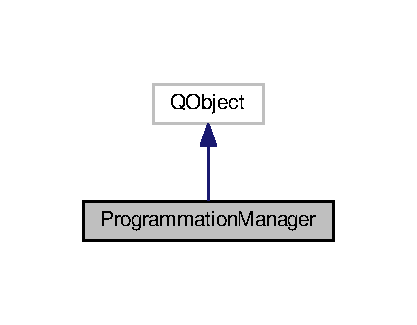
\includegraphics[width=200pt]{class_programmation_manager__inherit__graph}
\end{center}
\end{figure}


Collaboration diagram for Programmation\+Manager\+:\nopagebreak
\begin{figure}[H]
\begin{center}
\leavevmode
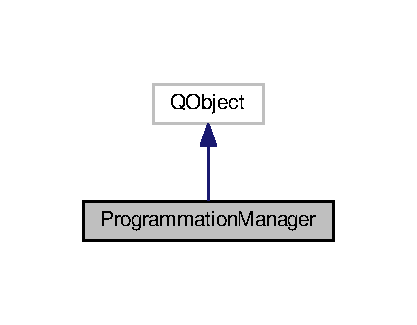
\includegraphics[width=200pt]{class_programmation_manager__coll__graph}
\end{center}
\end{figure}
\subsection*{Classes}
\begin{DoxyCompactItemize}
\item 
class \hyperlink{class_programmation_manager_1_1_iterator}{Iterator}
\end{DoxyCompactItemize}
\subsection*{Signals}
\begin{DoxyCompactItemize}
\item 
void \hyperlink{class_programmation_manager_ad6f6dbec484d80425f498460650a0649}{programmations\+Changed} ()
\begin{DoxyCompactList}\small\item\em Signal de changement de programmation. \end{DoxyCompactList}\end{DoxyCompactItemize}
\subsection*{Public Member Functions}
\begin{DoxyCompactItemize}
\item 
\hyperlink{class_programmation}{Programmation} $\ast$ \hyperlink{class_programmation_manager_a43fd958e37bf4a78b845006aa5551bec}{trouver\+Programmation} (\hyperlink{class_evenement}{Evenement} \&e) const 
\begin{DoxyCompactList}\small\item\em Renvoie le pointeur de la programmation de l\textquotesingle{}événement correspondant si elle existe dans le tableau. \end{DoxyCompactList}\item 
\hyperlink{class_programmation}{Programmation} $\ast$ \hyperlink{class_programmation_manager_ab52ba49ca1d79add9f6d83f8f9386b7e}{trouver\+Programmation} (const \hyperlink{class_evenement}{Evenement} \&e) const 
\begin{DoxyCompactList}\small\item\em Renvoie le pointeur de la programmation de l\textquotesingle{}événement const correspondant si elle existe dans le tableau. \end{DoxyCompactList}\item 
void \hyperlink{class_programmation_manager_a8b6067aba53b0389d30c485c9a544769}{ajouter\+Programmation} (\hyperlink{class_unitaire}{Unitaire} \&e, const \hyperlink{class_t_i_m_e_1_1_date}{Date} \&d, const \hyperlink{class_t_i_m_e_1_1_horaire}{Horaire} \&h, \hyperlink{class_t_i_m_e_1_1_duree}{Duree} dur)
\begin{DoxyCompactList}\small\item\em Crée une programmation d\textquotesingle{}une \hyperlink{class_tache}{Tache} \hyperlink{class_unitaire}{Unitaire} et stocke le pointeur dans le tableau programmations. \end{DoxyCompactList}\item 
void \hyperlink{class_programmation_manager_a3451eabd67b35163c6213eed9b2f3733}{ajouter\+Programmation} (\hyperlink{class_activite}{Activite} \&e, const \hyperlink{class_t_i_m_e_1_1_date}{Date} \&d, const \hyperlink{class_t_i_m_e_1_1_horaire}{Horaire} \&h, const \hyperlink{class_t_i_m_e_1_1_duree}{Duree} \&dur)
\begin{DoxyCompactList}\small\item\em Crée une programmation d\textquotesingle{}une Activité et stocke le pointeur dans le tableau programmations. \end{DoxyCompactList}\item 
\hyperlink{class_programmation_manager_1_1_iterator}{Iterator} \hyperlink{class_programmation_manager_aaff6e0852f9e7ec4aeb47f6ef976fdf9}{get\+Iterator} ()
\begin{DoxyCompactList}\small\item\em Renvoie un iterateur sur programmations. \end{DoxyCompactList}\end{DoxyCompactItemize}
\subsection*{Static Public Member Functions}
\begin{DoxyCompactItemize}
\item 
static \hyperlink{class_programmation_manager}{Programmation\+Manager} \& \hyperlink{class_programmation_manager_a9da2fc647972756d1f8cdf91d4017c25}{get\+Instance} ()
\begin{DoxyCompactList}\small\item\em Renvoie la seule instance de \hyperlink{class_programmation_manager}{Programmation\+Manager}. \end{DoxyCompactList}\item 
static void \hyperlink{class_programmation_manager_a94e3fcb28ea7c632dc6750c33949d712}{liberer\+Instance} ()
\begin{DoxyCompactList}\small\item\em Libère l\textquotesingle{}unique instance de \hyperlink{class_programmation_manager}{Programmation\+Manager}. \end{DoxyCompactList}\end{DoxyCompactItemize}


\subsection{Detailed Description}
Classe composite de \hyperlink{class_programmation}{Programmation} La classe applique le designe pattern singleton et possède un iterateur sur le tableau de pointeurs de Programmations. 

\subsection{Member Function Documentation}
\hypertarget{class_programmation_manager_a8b6067aba53b0389d30c485c9a544769}{}\index{Programmation\+Manager@{Programmation\+Manager}!ajouter\+Programmation@{ajouter\+Programmation}}
\index{ajouter\+Programmation@{ajouter\+Programmation}!Programmation\+Manager@{Programmation\+Manager}}
\subsubsection[{ajouter\+Programmation}]{\setlength{\rightskip}{0pt plus 5cm}void Programmation\+Manager\+::ajouter\+Programmation (
\begin{DoxyParamCaption}
\item[{{\bf Unitaire} \&}]{e, }
\item[{const {\bf Date} \&}]{d, }
\item[{const {\bf Horaire} \&}]{h, }
\item[{{\bf Duree}}]{dur}
\end{DoxyParamCaption}
)}\label{class_programmation_manager_a8b6067aba53b0389d30c485c9a544769}


Crée une programmation d\textquotesingle{}une \hyperlink{class_tache}{Tache} \hyperlink{class_unitaire}{Unitaire} et stocke le pointeur dans le tableau programmations. 

\hypertarget{class_programmation_manager_a3451eabd67b35163c6213eed9b2f3733}{}\index{Programmation\+Manager@{Programmation\+Manager}!ajouter\+Programmation@{ajouter\+Programmation}}
\index{ajouter\+Programmation@{ajouter\+Programmation}!Programmation\+Manager@{Programmation\+Manager}}
\subsubsection[{ajouter\+Programmation}]{\setlength{\rightskip}{0pt plus 5cm}void Programmation\+Manager\+::ajouter\+Programmation (
\begin{DoxyParamCaption}
\item[{{\bf Activite} \&}]{e, }
\item[{const {\bf Date} \&}]{d, }
\item[{const {\bf Horaire} \&}]{h, }
\item[{const {\bf Duree} \&}]{dur}
\end{DoxyParamCaption}
)}\label{class_programmation_manager_a3451eabd67b35163c6213eed9b2f3733}


Crée une programmation d\textquotesingle{}une Activité et stocke le pointeur dans le tableau programmations. 

\hypertarget{class_programmation_manager_a9da2fc647972756d1f8cdf91d4017c25}{}\index{Programmation\+Manager@{Programmation\+Manager}!get\+Instance@{get\+Instance}}
\index{get\+Instance@{get\+Instance}!Programmation\+Manager@{Programmation\+Manager}}
\subsubsection[{get\+Instance}]{\setlength{\rightskip}{0pt plus 5cm}{\bf Programmation\+Manager} \& Programmation\+Manager\+::get\+Instance (
\begin{DoxyParamCaption}
{}
\end{DoxyParamCaption}
)\hspace{0.3cm}{\ttfamily [static]}}\label{class_programmation_manager_a9da2fc647972756d1f8cdf91d4017c25}


Renvoie la seule instance de \hyperlink{class_programmation_manager}{Programmation\+Manager}. 

\hypertarget{class_programmation_manager_aaff6e0852f9e7ec4aeb47f6ef976fdf9}{}\index{Programmation\+Manager@{Programmation\+Manager}!get\+Iterator@{get\+Iterator}}
\index{get\+Iterator@{get\+Iterator}!Programmation\+Manager@{Programmation\+Manager}}
\subsubsection[{get\+Iterator}]{\setlength{\rightskip}{0pt plus 5cm}{\bf Iterator} Programmation\+Manager\+::get\+Iterator (
\begin{DoxyParamCaption}
{}
\end{DoxyParamCaption}
)\hspace{0.3cm}{\ttfamily [inline]}}\label{class_programmation_manager_aaff6e0852f9e7ec4aeb47f6ef976fdf9}


Renvoie un iterateur sur programmations. 

\hypertarget{class_programmation_manager_a94e3fcb28ea7c632dc6750c33949d712}{}\index{Programmation\+Manager@{Programmation\+Manager}!liberer\+Instance@{liberer\+Instance}}
\index{liberer\+Instance@{liberer\+Instance}!Programmation\+Manager@{Programmation\+Manager}}
\subsubsection[{liberer\+Instance}]{\setlength{\rightskip}{0pt plus 5cm}void Programmation\+Manager\+::liberer\+Instance (
\begin{DoxyParamCaption}
{}
\end{DoxyParamCaption}
)\hspace{0.3cm}{\ttfamily [static]}}\label{class_programmation_manager_a94e3fcb28ea7c632dc6750c33949d712}


Libère l\textquotesingle{}unique instance de \hyperlink{class_programmation_manager}{Programmation\+Manager}. 

\hypertarget{class_programmation_manager_ad6f6dbec484d80425f498460650a0649}{}\index{Programmation\+Manager@{Programmation\+Manager}!programmations\+Changed@{programmations\+Changed}}
\index{programmations\+Changed@{programmations\+Changed}!Programmation\+Manager@{Programmation\+Manager}}
\subsubsection[{programmations\+Changed}]{\setlength{\rightskip}{0pt plus 5cm}void Programmation\+Manager\+::programmations\+Changed (
\begin{DoxyParamCaption}
{}
\end{DoxyParamCaption}
)\hspace{0.3cm}{\ttfamily [signal]}}\label{class_programmation_manager_ad6f6dbec484d80425f498460650a0649}


Signal de changement de programmation. 

\hypertarget{class_programmation_manager_a43fd958e37bf4a78b845006aa5551bec}{}\index{Programmation\+Manager@{Programmation\+Manager}!trouver\+Programmation@{trouver\+Programmation}}
\index{trouver\+Programmation@{trouver\+Programmation}!Programmation\+Manager@{Programmation\+Manager}}
\subsubsection[{trouver\+Programmation}]{\setlength{\rightskip}{0pt plus 5cm}{\bf Programmation} $\ast$ Programmation\+Manager\+::trouver\+Programmation (
\begin{DoxyParamCaption}
\item[{{\bf Evenement} \&}]{e}
\end{DoxyParamCaption}
) const}\label{class_programmation_manager_a43fd958e37bf4a78b845006aa5551bec}


Renvoie le pointeur de la programmation de l\textquotesingle{}événement correspondant si elle existe dans le tableau. 

\hypertarget{class_programmation_manager_ab52ba49ca1d79add9f6d83f8f9386b7e}{}\index{Programmation\+Manager@{Programmation\+Manager}!trouver\+Programmation@{trouver\+Programmation}}
\index{trouver\+Programmation@{trouver\+Programmation}!Programmation\+Manager@{Programmation\+Manager}}
\subsubsection[{trouver\+Programmation}]{\setlength{\rightskip}{0pt plus 5cm}{\bf Programmation} $\ast$ Programmation\+Manager\+::trouver\+Programmation (
\begin{DoxyParamCaption}
\item[{const {\bf Evenement} \&}]{e}
\end{DoxyParamCaption}
) const}\label{class_programmation_manager_ab52ba49ca1d79add9f6d83f8f9386b7e}


Renvoie le pointeur de la programmation de l\textquotesingle{}événement const correspondant si elle existe dans le tableau. 



The documentation for this class was generated from the following files\+:\begin{DoxyCompactItemize}
\item 
L\+O21app/\hyperlink{_calendar_8h}{Calendar.\+h}\item 
L\+O21app/\hyperlink{_calendar_8cpp}{Calendar.\+cpp}\end{DoxyCompactItemize}

\hypertarget{class_projet}{}\section{Projet Class Reference}
\label{class_projet}\index{Projet@{Projet}}


Un ensemble de tache à réaliser.  




{\ttfamily \#include $<$Calendar.\+h$>$}

\subsection*{Classes}
\begin{DoxyCompactItemize}
\item 
class \hyperlink{class_projet_1_1_iterator}{Iterator}
\end{DoxyCompactItemize}
\subsection*{Public Member Functions}
\begin{DoxyCompactItemize}
\item 
\hypertarget{class_projet_abc4ef9586bab910e754d4f88943df720}{}string \hyperlink{class_projet_abc4ef9586bab910e754d4f88943df720}{get\+Nom} () const \label{class_projet_abc4ef9586bab910e754d4f88943df720}

\begin{DoxyCompactList}\small\item\em accesseur \end{DoxyCompactList}\item 
\hypertarget{class_projet_acb3ac5233074e53f0263bd50b4e0bdec}{}\hyperlink{class_projet_1_1_iterator}{Iterator} {\bfseries get\+Iterator} ()\label{class_projet_acb3ac5233074e53f0263bd50b4e0bdec}

\end{DoxyCompactItemize}
\subsection*{Friends}
\begin{DoxyCompactItemize}
\item 
\hypertarget{class_projet_a9830fc407400559db7e7783cc10a9394}{}class {\bfseries Iterator}\label{class_projet_a9830fc407400559db7e7783cc10a9394}

\end{DoxyCompactItemize}


\subsection{Detailed Description}
Un ensemble de tache à réaliser. 

The documentation for this class was generated from the following file\+:\begin{DoxyCompactItemize}
\item 
L\+O21app/Calendar.\+h\end{DoxyCompactItemize}

\hypertarget{class_tache}{}\section{Tache Class Reference}
\label{class_tache}\index{Tache@{Tache}}


Classe abstraite de taches composant \hyperlink{class_projet}{Projet}.  




{\ttfamily \#include $<$Calendar.\+h$>$}



Inheritance diagram for Tache\+:\nopagebreak
\begin{figure}[H]
\begin{center}
\leavevmode
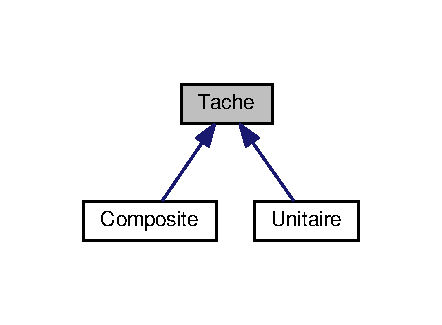
\includegraphics[width=212pt]{class_tache__inherit__graph}
\end{center}
\end{figure}
\subsection*{Classes}
\begin{DoxyCompactItemize}
\item 
class \hyperlink{class_tache_1_1_iterator}{Iterator}
\end{DoxyCompactItemize}
\subsection*{Public Member Functions}
\begin{DoxyCompactItemize}
\item 
unsigned int \hyperlink{class_tache_ac597ce580ad0b32c373b329d4da839ad}{get\+Nb\+Pred} ()
\begin{DoxyCompactList}\small\item\em Renvoie le nombre d\textquotesingle{}éléments de prec. \end{DoxyCompactList}\item 
\hyperlink{class_projet}{Projet} $\ast$ \hyperlink{class_tache_aa6d1abc3712b5a8b571bb3c131129ac7}{get\+Projet} () const 
\begin{DoxyCompactList}\small\item\em Renvoie un pointeur vers le projet parent de la tache. \end{DoxyCompactList}\item 
virtual \hyperlink{class_tache_acefc2a88516ef4d8bd7b25afcf769e9c}{$\sim$\+Tache} ()
\begin{DoxyCompactList}\small\item\em Desctructeur de la tache. \end{DoxyCompactList}\item 
\hyperlink{class_tache_a026b068c4e49643d6fec30c9b915ddca}{Tache} (const string \&id, const string \&t, const \hyperlink{class_t_i_m_e_1_1_date}{Date} \&dispo, const \hyperlink{class_t_i_m_e_1_1_date}{Date} \&deadline, \hyperlink{class_projet}{Projet} $\ast$p)
\item 
virtual void \hyperlink{class_tache_a6a13b4138a46f22e632bf9d35f155c09}{add\+Item} (\hyperlink{class_tache}{Tache} $\ast$t)
\begin{DoxyCompactList}\small\item\em Ajoute le pointeur de tache dans prec comme nouvelle contrainte de précédence. \end{DoxyCompactList}\item 
\hyperlink{class_tache}{Tache} \& \hyperlink{class_tache_ab29bfb6c79337fbc9dc5618195f12f8d}{get\+Precedence} (const string \&id)
\begin{DoxyCompactList}\small\item\em Renvoie une référence vers la tache désignée par id si elle existe dans prec. \end{DoxyCompactList}\item 
const \hyperlink{class_tache}{Tache} \& \hyperlink{class_tache_af995526e12eed76ffa2a4ba7b6fb7a90}{get\+Precedence} (const string \&code) const 
\begin{DoxyCompactList}\small\item\em Renvoie une const référence vers la tache désignée par id si elle existe dans prec. \end{DoxyCompactList}\item 
bool \hyperlink{class_tache_a72df18190512de6ca437492a3664d05a}{is\+Precedence} () const 
\begin{DoxyCompactList}\small\item\em Indique par booléen si la tache a des précédences ou non. \end{DoxyCompactList}\item 
virtual bool \hyperlink{class_tache_ae873dc0bfe552ea39c34f430d56f3846}{is\+Precedence\+Potentielle} (const string \&id)
\begin{DoxyCompactList}\small\item\em Indique si la tache désignée par id est une précédence potentielle ou non pour la tache. \end{DoxyCompactList}\item 
string \hyperlink{class_tache_a1fe8754733f0b85c232d91851cf61891}{get\+Id} () const 
\begin{DoxyCompactList}\small\item\em Renvoie l\textquotesingle{}identificateur de la tache. \end{DoxyCompactList}\item 
string \hyperlink{class_tache_ab6af5354e29498ab43ab3cc826b0aac4}{get\+Titre} () const 
\begin{DoxyCompactList}\small\item\em Renvoie le titre de la tache. \end{DoxyCompactList}\item 
\hyperlink{class_t_i_m_e_1_1_date}{Date} \hyperlink{class_tache_a8cba5e74f4ee6b31e29d0339dbe470fe}{get\+Date\+Disponibilite} () const 
\begin{DoxyCompactList}\small\item\em Renvoie la date de disponibilité de la tache. \end{DoxyCompactList}\item 
\hyperlink{class_t_i_m_e_1_1_date}{Date} \hyperlink{class_tache_abe0dbe94fc6908ba5e3cb7fd2fa90f92}{get\+Date\+Echeance} () const 
\begin{DoxyCompactList}\small\item\em Renvoie la date d\textquotesingle{}échéance de la tache. \end{DoxyCompactList}\item 
\hyperlink{class_projet}{Projet} $\ast$ \hyperlink{class_tache_a18bda9873a4643a7bebe4905110e3814}{get\+Projet} ()
\begin{DoxyCompactList}\small\item\em Renvoie le pointeur vers le projet parent. \end{DoxyCompactList}\item 
virtual int \hyperlink{class_tache_ac60426a56aec80b995f30456fc60a256}{get\+Statut} ()=0
\begin{DoxyCompactList}\small\item\em Retourne le statut de la tache \+: 0 = rien n\textquotesingle{}est fait, 1 = en cours, 2 = terminé/deadline passée. \end{DoxyCompactList}\item 
virtual int \hyperlink{class_tache_a495d9d787ef400a510e625e4e51014bd}{is\+Finished} (const \hyperlink{class_t_i_m_e_1_1_date}{Date} \&d, const \hyperlink{class_t_i_m_e_1_1_horaire}{Horaire} \&h)=0
\begin{DoxyCompactList}\small\item\em Renvoie 1 si la tache a été terminée à la date d et l\textquotesingle{}horaire h, 0 sinon. \end{DoxyCompactList}\item 
void \hyperlink{class_tache_a4ea66e1007e692875199d4027e724a85}{set\+Id} (const string \&id)
\begin{DoxyCompactList}\small\item\em Modifie l\textquotesingle{}identificateur. \end{DoxyCompactList}\item 
void \hyperlink{class_tache_a191acd8b10c22b8e7a533aa8f237b907}{set\+Titre} (const string \&t)
\begin{DoxyCompactList}\small\item\em Modifie le titre. \end{DoxyCompactList}\item 
void \hyperlink{class_tache_a56de6bd26a4a5028c01481ccdededd54}{set\+Dates\+Disponibilite\+Echeance} (const \hyperlink{class_t_i_m_e_1_1_date}{Date} \&disp, const \hyperlink{class_t_i_m_e_1_1_date}{Date} \&e)
\item 
\hyperlink{class_tache_1_1_iterator}{Iterator} \hyperlink{class_tache_a709d4d7d5c25604b6e9a5c37b74fa4a6}{get\+Iterator} ()
\begin{DoxyCompactList}\small\item\em Renvoie un itérateur sur prec. \end{DoxyCompactList}\item 
virtual void \hyperlink{class_tache_a2f86a1a329eb7eee7c8ef4491439bc1c}{afficher} (ostream \&f)=0
\begin{DoxyCompactList}\small\item\em Méthode virtuelle pure d\textquotesingle{}affichage de la tache. \end{DoxyCompactList}\end{DoxyCompactItemize}


\subsection{Detailed Description}
Classe abstraite de taches composant \hyperlink{class_projet}{Projet}. 

\subsection{Constructor \& Destructor Documentation}
\hypertarget{class_tache_acefc2a88516ef4d8bd7b25afcf769e9c}{}\index{Tache@{Tache}!````~Tache@{$\sim$\+Tache}}
\index{````~Tache@{$\sim$\+Tache}!Tache@{Tache}}
\subsubsection[{$\sim$\+Tache}]{\setlength{\rightskip}{0pt plus 5cm}virtual Tache\+::$\sim$\+Tache (
\begin{DoxyParamCaption}
{}
\end{DoxyParamCaption}
)\hspace{0.3cm}{\ttfamily [inline]}, {\ttfamily [virtual]}}\label{class_tache_acefc2a88516ef4d8bd7b25afcf769e9c}


Desctructeur de la tache. 

\hypertarget{class_tache_a026b068c4e49643d6fec30c9b915ddca}{}\index{Tache@{Tache}!Tache@{Tache}}
\index{Tache@{Tache}!Tache@{Tache}}
\subsubsection[{Tache}]{\setlength{\rightskip}{0pt plus 5cm}Tache\+::\+Tache (
\begin{DoxyParamCaption}
\item[{const string \&}]{id, }
\item[{const string \&}]{t, }
\item[{const {\bf Date} \&}]{dispo, }
\item[{const {\bf Date} \&}]{deadline, }
\item[{{\bf Projet} $\ast$}]{p}
\end{DoxyParamCaption}
)\hspace{0.3cm}{\ttfamily [inline]}}\label{class_tache_a026b068c4e49643d6fec30c9b915ddca}


\subsection{Member Function Documentation}
\hypertarget{class_tache_a6a13b4138a46f22e632bf9d35f155c09}{}\index{Tache@{Tache}!add\+Item@{add\+Item}}
\index{add\+Item@{add\+Item}!Tache@{Tache}}
\subsubsection[{add\+Item}]{\setlength{\rightskip}{0pt plus 5cm}void Tache\+::add\+Item (
\begin{DoxyParamCaption}
\item[{{\bf Tache} $\ast$}]{t}
\end{DoxyParamCaption}
)\hspace{0.3cm}{\ttfamily [virtual]}}\label{class_tache_a6a13b4138a46f22e632bf9d35f155c09}


Ajoute le pointeur de tache dans prec comme nouvelle contrainte de précédence. 



Reimplemented in \hyperlink{class_composite_ab0d63970716648141fbc24e7d77815a2}{Composite}, and \hyperlink{class_unitaire_a804454c39eb010aa67bd622a009df840}{Unitaire}.

\hypertarget{class_tache_a2f86a1a329eb7eee7c8ef4491439bc1c}{}\index{Tache@{Tache}!afficher@{afficher}}
\index{afficher@{afficher}!Tache@{Tache}}
\subsubsection[{afficher}]{\setlength{\rightskip}{0pt plus 5cm}virtual void Tache\+::afficher (
\begin{DoxyParamCaption}
\item[{ostream \&}]{f}
\end{DoxyParamCaption}
)\hspace{0.3cm}{\ttfamily [pure virtual]}}\label{class_tache_a2f86a1a329eb7eee7c8ef4491439bc1c}


Méthode virtuelle pure d\textquotesingle{}affichage de la tache. 



Implemented in \hyperlink{class_composite_a36da340a18bdf872a180c9657c5996c2}{Composite}, and \hyperlink{class_unitaire_a98bd645b84e0bd2f378e13774324f7b7}{Unitaire}.

\hypertarget{class_tache_a8cba5e74f4ee6b31e29d0339dbe470fe}{}\index{Tache@{Tache}!get\+Date\+Disponibilite@{get\+Date\+Disponibilite}}
\index{get\+Date\+Disponibilite@{get\+Date\+Disponibilite}!Tache@{Tache}}
\subsubsection[{get\+Date\+Disponibilite}]{\setlength{\rightskip}{0pt plus 5cm}{\bf Date} Tache\+::get\+Date\+Disponibilite (
\begin{DoxyParamCaption}
{}
\end{DoxyParamCaption}
) const\hspace{0.3cm}{\ttfamily [inline]}}\label{class_tache_a8cba5e74f4ee6b31e29d0339dbe470fe}


Renvoie la date de disponibilité de la tache. 

\hypertarget{class_tache_abe0dbe94fc6908ba5e3cb7fd2fa90f92}{}\index{Tache@{Tache}!get\+Date\+Echeance@{get\+Date\+Echeance}}
\index{get\+Date\+Echeance@{get\+Date\+Echeance}!Tache@{Tache}}
\subsubsection[{get\+Date\+Echeance}]{\setlength{\rightskip}{0pt plus 5cm}{\bf Date} Tache\+::get\+Date\+Echeance (
\begin{DoxyParamCaption}
{}
\end{DoxyParamCaption}
) const\hspace{0.3cm}{\ttfamily [inline]}}\label{class_tache_abe0dbe94fc6908ba5e3cb7fd2fa90f92}


Renvoie la date d\textquotesingle{}échéance de la tache. 

\hypertarget{class_tache_a1fe8754733f0b85c232d91851cf61891}{}\index{Tache@{Tache}!get\+Id@{get\+Id}}
\index{get\+Id@{get\+Id}!Tache@{Tache}}
\subsubsection[{get\+Id}]{\setlength{\rightskip}{0pt plus 5cm}string Tache\+::get\+Id (
\begin{DoxyParamCaption}
{}
\end{DoxyParamCaption}
) const\hspace{0.3cm}{\ttfamily [inline]}}\label{class_tache_a1fe8754733f0b85c232d91851cf61891}


Renvoie l\textquotesingle{}identificateur de la tache. 

\hypertarget{class_tache_a709d4d7d5c25604b6e9a5c37b74fa4a6}{}\index{Tache@{Tache}!get\+Iterator@{get\+Iterator}}
\index{get\+Iterator@{get\+Iterator}!Tache@{Tache}}
\subsubsection[{get\+Iterator}]{\setlength{\rightskip}{0pt plus 5cm}{\bf Iterator} Tache\+::get\+Iterator (
\begin{DoxyParamCaption}
{}
\end{DoxyParamCaption}
)\hspace{0.3cm}{\ttfamily [inline]}}\label{class_tache_a709d4d7d5c25604b6e9a5c37b74fa4a6}


Renvoie un itérateur sur prec. 

\hypertarget{class_tache_ac597ce580ad0b32c373b329d4da839ad}{}\index{Tache@{Tache}!get\+Nb\+Pred@{get\+Nb\+Pred}}
\index{get\+Nb\+Pred@{get\+Nb\+Pred}!Tache@{Tache}}
\subsubsection[{get\+Nb\+Pred}]{\setlength{\rightskip}{0pt plus 5cm}unsigned int Tache\+::get\+Nb\+Pred (
\begin{DoxyParamCaption}
{}
\end{DoxyParamCaption}
)\hspace{0.3cm}{\ttfamily [inline]}}\label{class_tache_ac597ce580ad0b32c373b329d4da839ad}


Renvoie le nombre d\textquotesingle{}éléments de prec. 

\hypertarget{class_tache_ab29bfb6c79337fbc9dc5618195f12f8d}{}\index{Tache@{Tache}!get\+Precedence@{get\+Precedence}}
\index{get\+Precedence@{get\+Precedence}!Tache@{Tache}}
\subsubsection[{get\+Precedence}]{\setlength{\rightskip}{0pt plus 5cm}{\bf Tache} \& Tache\+::get\+Precedence (
\begin{DoxyParamCaption}
\item[{const string \&}]{id}
\end{DoxyParamCaption}
)}\label{class_tache_ab29bfb6c79337fbc9dc5618195f12f8d}


Renvoie une référence vers la tache désignée par id si elle existe dans prec. 

\hypertarget{class_tache_af995526e12eed76ffa2a4ba7b6fb7a90}{}\index{Tache@{Tache}!get\+Precedence@{get\+Precedence}}
\index{get\+Precedence@{get\+Precedence}!Tache@{Tache}}
\subsubsection[{get\+Precedence}]{\setlength{\rightskip}{0pt plus 5cm}const {\bf Tache} \& Tache\+::get\+Precedence (
\begin{DoxyParamCaption}
\item[{const string \&}]{code}
\end{DoxyParamCaption}
) const}\label{class_tache_af995526e12eed76ffa2a4ba7b6fb7a90}


Renvoie une const référence vers la tache désignée par id si elle existe dans prec. 

\hypertarget{class_tache_aa6d1abc3712b5a8b571bb3c131129ac7}{}\index{Tache@{Tache}!get\+Projet@{get\+Projet}}
\index{get\+Projet@{get\+Projet}!Tache@{Tache}}
\subsubsection[{get\+Projet}]{\setlength{\rightskip}{0pt plus 5cm}{\bf Projet}$\ast$ Tache\+::get\+Projet (
\begin{DoxyParamCaption}
{}
\end{DoxyParamCaption}
) const\hspace{0.3cm}{\ttfamily [inline]}}\label{class_tache_aa6d1abc3712b5a8b571bb3c131129ac7}


Renvoie un pointeur vers le projet parent de la tache. 

\hypertarget{class_tache_a18bda9873a4643a7bebe4905110e3814}{}\index{Tache@{Tache}!get\+Projet@{get\+Projet}}
\index{get\+Projet@{get\+Projet}!Tache@{Tache}}
\subsubsection[{get\+Projet}]{\setlength{\rightskip}{0pt plus 5cm}{\bf Projet}$\ast$ Tache\+::get\+Projet (
\begin{DoxyParamCaption}
{}
\end{DoxyParamCaption}
)\hspace{0.3cm}{\ttfamily [inline]}}\label{class_tache_a18bda9873a4643a7bebe4905110e3814}


Renvoie le pointeur vers le projet parent. 

\hypertarget{class_tache_ac60426a56aec80b995f30456fc60a256}{}\index{Tache@{Tache}!get\+Statut@{get\+Statut}}
\index{get\+Statut@{get\+Statut}!Tache@{Tache}}
\subsubsection[{get\+Statut}]{\setlength{\rightskip}{0pt plus 5cm}virtual int Tache\+::get\+Statut (
\begin{DoxyParamCaption}
{}
\end{DoxyParamCaption}
)\hspace{0.3cm}{\ttfamily [pure virtual]}}\label{class_tache_ac60426a56aec80b995f30456fc60a256}


Retourne le statut de la tache \+: 0 = rien n\textquotesingle{}est fait, 1 = en cours, 2 = terminé/deadline passée. 



Implemented in \hyperlink{class_composite_a6def8410e8a78678b488d1610266ee5b}{Composite}, and \hyperlink{class_unitaire_aadf6c5718aff37f1a7589240059e9e98}{Unitaire}.

\hypertarget{class_tache_ab6af5354e29498ab43ab3cc826b0aac4}{}\index{Tache@{Tache}!get\+Titre@{get\+Titre}}
\index{get\+Titre@{get\+Titre}!Tache@{Tache}}
\subsubsection[{get\+Titre}]{\setlength{\rightskip}{0pt plus 5cm}string Tache\+::get\+Titre (
\begin{DoxyParamCaption}
{}
\end{DoxyParamCaption}
) const\hspace{0.3cm}{\ttfamily [inline]}}\label{class_tache_ab6af5354e29498ab43ab3cc826b0aac4}


Renvoie le titre de la tache. 

\hypertarget{class_tache_a495d9d787ef400a510e625e4e51014bd}{}\index{Tache@{Tache}!is\+Finished@{is\+Finished}}
\index{is\+Finished@{is\+Finished}!Tache@{Tache}}
\subsubsection[{is\+Finished}]{\setlength{\rightskip}{0pt plus 5cm}virtual int Tache\+::is\+Finished (
\begin{DoxyParamCaption}
\item[{const {\bf Date} \&}]{d, }
\item[{const {\bf Horaire} \&}]{h}
\end{DoxyParamCaption}
)\hspace{0.3cm}{\ttfamily [pure virtual]}}\label{class_tache_a495d9d787ef400a510e625e4e51014bd}


Renvoie 1 si la tache a été terminée à la date d et l\textquotesingle{}horaire h, 0 sinon. 



Implemented in \hyperlink{class_composite_a4dd23b6bafdc87f05f0cb7d19e459f94}{Composite}, and \hyperlink{class_unitaire_affee1a6cda05a1032eba560196af99b9}{Unitaire}.

\hypertarget{class_tache_a72df18190512de6ca437492a3664d05a}{}\index{Tache@{Tache}!is\+Precedence@{is\+Precedence}}
\index{is\+Precedence@{is\+Precedence}!Tache@{Tache}}
\subsubsection[{is\+Precedence}]{\setlength{\rightskip}{0pt plus 5cm}bool Tache\+::is\+Precedence (
\begin{DoxyParamCaption}
{}
\end{DoxyParamCaption}
) const\hspace{0.3cm}{\ttfamily [inline]}}\label{class_tache_a72df18190512de6ca437492a3664d05a}


Indique par booléen si la tache a des précédences ou non. 

\hypertarget{class_tache_ae873dc0bfe552ea39c34f430d56f3846}{}\index{Tache@{Tache}!is\+Precedence\+Potentielle@{is\+Precedence\+Potentielle}}
\index{is\+Precedence\+Potentielle@{is\+Precedence\+Potentielle}!Tache@{Tache}}
\subsubsection[{is\+Precedence\+Potentielle}]{\setlength{\rightskip}{0pt plus 5cm}bool Tache\+::is\+Precedence\+Potentielle (
\begin{DoxyParamCaption}
\item[{const string \&}]{id}
\end{DoxyParamCaption}
)\hspace{0.3cm}{\ttfamily [virtual]}}\label{class_tache_ae873dc0bfe552ea39c34f430d56f3846}


Indique si la tache désignée par id est une précédence potentielle ou non pour la tache. 



Reimplemented in \hyperlink{class_composite_a38fbb5005db8a763fec1c8c04f63e1e0}{Composite}.

\hypertarget{class_tache_a56de6bd26a4a5028c01481ccdededd54}{}\index{Tache@{Tache}!set\+Dates\+Disponibilite\+Echeance@{set\+Dates\+Disponibilite\+Echeance}}
\index{set\+Dates\+Disponibilite\+Echeance@{set\+Dates\+Disponibilite\+Echeance}!Tache@{Tache}}
\subsubsection[{set\+Dates\+Disponibilite\+Echeance}]{\setlength{\rightskip}{0pt plus 5cm}void Tache\+::set\+Dates\+Disponibilite\+Echeance (
\begin{DoxyParamCaption}
\item[{const {\bf Date} \&}]{disp, }
\item[{const {\bf Date} \&}]{e}
\end{DoxyParamCaption}
)\hspace{0.3cm}{\ttfamily [inline]}}\label{class_tache_a56de6bd26a4a5028c01481ccdededd54}
Modifie les dates de disponibilité et d\textquotesingle{}échéance de la tache si elles sont compatibles \hypertarget{class_tache_a4ea66e1007e692875199d4027e724a85}{}\index{Tache@{Tache}!set\+Id@{set\+Id}}
\index{set\+Id@{set\+Id}!Tache@{Tache}}
\subsubsection[{set\+Id}]{\setlength{\rightskip}{0pt plus 5cm}void Tache\+::set\+Id (
\begin{DoxyParamCaption}
\item[{const string \&}]{id}
\end{DoxyParamCaption}
)\hspace{0.3cm}{\ttfamily [inline]}}\label{class_tache_a4ea66e1007e692875199d4027e724a85}


Modifie l\textquotesingle{}identificateur. 

\hypertarget{class_tache_a191acd8b10c22b8e7a533aa8f237b907}{}\index{Tache@{Tache}!set\+Titre@{set\+Titre}}
\index{set\+Titre@{set\+Titre}!Tache@{Tache}}
\subsubsection[{set\+Titre}]{\setlength{\rightskip}{0pt plus 5cm}void Tache\+::set\+Titre (
\begin{DoxyParamCaption}
\item[{const string \&}]{t}
\end{DoxyParamCaption}
)\hspace{0.3cm}{\ttfamily [inline]}}\label{class_tache_a191acd8b10c22b8e7a533aa8f237b907}


Modifie le titre. 



The documentation for this class was generated from the following files\+:\begin{DoxyCompactItemize}
\item 
L\+O21app/\hyperlink{_calendar_8h}{Calendar.\+h}\item 
L\+O21app/\hyperlink{_calendar_8cpp}{Calendar.\+cpp}\end{DoxyCompactItemize}

\hypertarget{class_t_i_m_e_1_1_time_exception}{}\section{T\+I\+M\+E\+:\+:Time\+Exception Class Reference}
\label{class_t_i_m_e_1_1_time_exception}\index{T\+I\+M\+E\+::\+Time\+Exception@{T\+I\+M\+E\+::\+Time\+Exception}}


Classe permettant de g�rer les exceptions des classes du namespace T\+I\+M\+E.  




{\ttfamily \#include $<$timing.\+h$>$}

\subsection*{Public Member Functions}
\begin{DoxyCompactItemize}
\item 
\hypertarget{class_t_i_m_e_1_1_time_exception_a08502d82065dd79b27cd954b45f4d5c7}{}\hyperlink{class_t_i_m_e_1_1_time_exception_a08502d82065dd79b27cd954b45f4d5c7}{Time\+Exception} (const std\+::string \&m)\label{class_t_i_m_e_1_1_time_exception_a08502d82065dd79b27cd954b45f4d5c7}

\begin{DoxyCompactList}\small\item\em Constructeur � partir d\textquotesingle{}une string. \end{DoxyCompactList}\item 
\hypertarget{class_t_i_m_e_1_1_time_exception_ad86c212253ea1b8654f4cae34611d634}{}const std\+::string \& {\bfseries Get\+Info} () const \label{class_t_i_m_e_1_1_time_exception_ad86c212253ea1b8654f4cae34611d634}

\end{DoxyCompactItemize}


\subsection{Detailed Description}
Classe permettant de g�rer les exceptions des classes du namespace T\+I\+M\+E. 

The documentation for this class was generated from the following file\+:\begin{DoxyCompactItemize}
\item 
L\+O21app/timing.\+h\end{DoxyCompactItemize}

\hypertarget{class_truc}{}\section{Truc Class Reference}
\label{class_truc}\index{Truc@{Truc}}


Inheritance diagram for Truc\+:\nopagebreak
\begin{figure}[H]
\begin{center}
\leavevmode
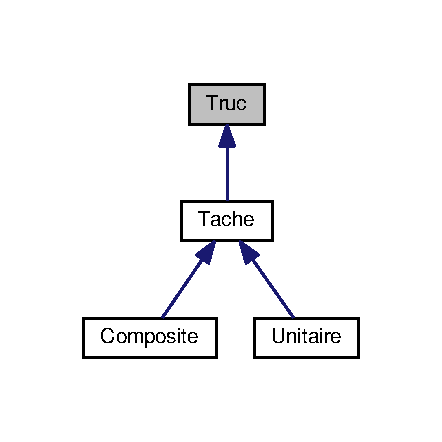
\includegraphics[width=212pt]{class_truc__inherit__graph}
\end{center}
\end{figure}


Collaboration diagram for Truc\+:\nopagebreak
\begin{figure}[H]
\begin{center}
\leavevmode
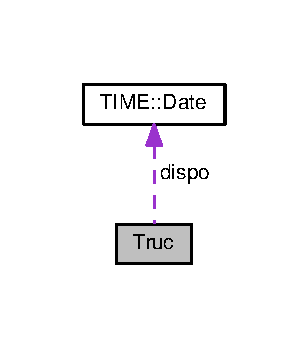
\includegraphics[width=148pt]{class_truc__coll__graph}
\end{center}
\end{figure}
\subsection*{Public Member Functions}
\begin{DoxyCompactItemize}
\item 
\hypertarget{class_truc_aca95e48d9dc4a28745998319c0fb6233}{}\hyperlink{class_t_i_m_e_1_1_date}{Date} {\bfseries get\+Dispo} () const \label{class_truc_aca95e48d9dc4a28745998319c0fb6233}

\end{DoxyCompactItemize}
\subsection*{Public Attributes}
\begin{DoxyCompactItemize}
\item 
\hypertarget{class_truc_ab9df6defd6396fa46d998df1556645b6}{}\hyperlink{class_t_i_m_e_1_1_date}{Date} {\bfseries dispo}\label{class_truc_ab9df6defd6396fa46d998df1556645b6}

\end{DoxyCompactItemize}


The documentation for this class was generated from the following file\+:\begin{DoxyCompactItemize}
\item 
L\+O21app/Calendar.\+h\end{DoxyCompactItemize}

\hypertarget{class_unitaire}{}\section{Unitaire Class Reference}
\label{class_unitaire}\index{Unitaire@{Unitaire}}


Classe de taches programmables, héritant de Tachet et d\textquotesingle{}\hyperlink{class_evenement}{Evenement} La classe de taches pouvant être programmées, en plusieurs fois si préemptive, en une seule fois sinon. La classe est forcément préemptive si sa durée dépasse 12h.  




{\ttfamily \#include $<$Calendar.\+h$>$}



Inheritance diagram for Unitaire\+:\nopagebreak
\begin{figure}[H]
\begin{center}
\leavevmode
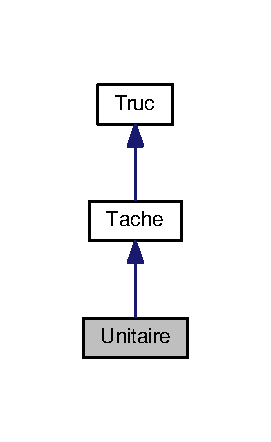
\includegraphics[width=208pt]{class_unitaire__inherit__graph}
\end{center}
\end{figure}


Collaboration diagram for Unitaire\+:\nopagebreak
\begin{figure}[H]
\begin{center}
\leavevmode
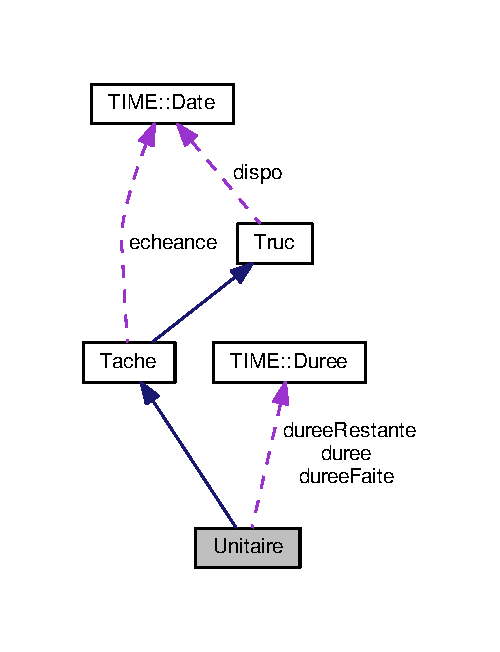
\includegraphics[width=208pt]{class_unitaire__coll__graph}
\end{center}
\end{figure}
\subsection*{Public Member Functions}
\begin{DoxyCompactItemize}
\item 
virtual void \hyperlink{class_unitaire_a804454c39eb010aa67bd622a009df840}{add\+Item} (\hyperlink{class_tache}{Tache} $\ast$t)
\begin{DoxyCompactList}\small\item\em Ajoute la tache pointée aux tableau de précédences prec. \end{DoxyCompactList}\item 
bool \hyperlink{class_unitaire_adba3a8de0fe6273cea7eecda3520bfcd}{is\+Preemp} () const 
\begin{DoxyCompactList}\small\item\em Indique si la tache est préemptable ou non. \end{DoxyCompactList}\item 
\hyperlink{class_t_i_m_e_1_1_duree}{Duree} \hyperlink{class_unitaire_a9ab243102aa0572048a956204532b201}{get\+Fait} () const 
\begin{DoxyCompactList}\small\item\em Retourne la durée faite de la tache. \end{DoxyCompactList}\item 
\hyperlink{class_t_i_m_e_1_1_duree}{Duree} \hyperlink{class_unitaire_a2fa3fa1073200a18c9a2706b37eb78e6}{get\+Restant} () const 
\begin{DoxyCompactList}\small\item\em Retourne la durée restante à programmer de la tache, calculée en soustrayant la durée totale avec la dutée faite. \end{DoxyCompactList}\item 
int \hyperlink{class_unitaire_aadf6c5718aff37f1a7589240059e9e98}{get\+Statut} ()
\begin{DoxyCompactList}\small\item\em Retourne le statut de la tache \+: 0 = rien n\textquotesingle{}est fait, 1 = en cours, 2 = terminé/deadline passée. \end{DoxyCompactList}\item 
virtual int \hyperlink{class_unitaire_affee1a6cda05a1032eba560196af99b9}{is\+Finished} (const \hyperlink{class_t_i_m_e_1_1_date}{Date} \&d, const \hyperlink{class_t_i_m_e_1_1_horaire}{Horaire} \&h)
\begin{DoxyCompactList}\small\item\em Renvoie 1 si la tache a été terminée à la date d et l\textquotesingle{}horaire h, 0 sinon. \end{DoxyCompactList}\item 
void \hyperlink{class_unitaire_ad9ef9d9bb2b47520c3c609d822364964}{set\+Fait} (const \hyperlink{class_t_i_m_e_1_1_duree}{Duree} \&f)
\begin{DoxyCompactList}\small\item\em Modifie la durée faite de la tache. \end{DoxyCompactList}\item 
void \hyperlink{class_unitaire_aa4893599f98385c26884441655331bc2}{set\+Preemp} ()
\begin{DoxyCompactList}\small\item\em Rend la tache préemptable. \end{DoxyCompactList}\item 
void \hyperlink{class_unitaire_a8bb9a65dc5b0d03a44353edfae06580d}{set\+Non\+Preemp} ()
\begin{DoxyCompactList}\small\item\em Rend, si possible, la tache preemptable. \end{DoxyCompactList}\item 
virtual void \hyperlink{class_unitaire_a98bd645b84e0bd2f378e13774324f7b7}{afficher} (ostream \&f)
\begin{DoxyCompactList}\small\item\em Affiche les attributs de la tache. \end{DoxyCompactList}\item 
void \hyperlink{class_unitaire_a965c3d4d8ba7864ae28a24a5d514dec5}{update} (string id, string t, \hyperlink{class_t_i_m_e_1_1_date}{Date} d, \hyperlink{class_t_i_m_e_1_1_date}{Date} e, \hyperlink{class_t_i_m_e_1_1_duree}{Duree} dur, \hyperlink{class_t_i_m_e_1_1_duree}{Duree} df, bool p)
\item 
void \hyperlink{class_unitaire_a2f189cf8c1bc7d22b805e6bfd1aa0bd7}{update} (string t, \hyperlink{class_t_i_m_e_1_1_date}{Date} d, \hyperlink{class_t_i_m_e_1_1_date}{Date} e, \hyperlink{class_t_i_m_e_1_1_duree}{Duree} dur, bool p)
\end{DoxyCompactItemize}
\subsection*{Friends}
\begin{DoxyCompactItemize}
\item 
\hyperlink{class_unitaire}{Unitaire} \& \hyperlink{class_unitaire_af32ab372e13abfb17b253ade6390cfd3}{Projet\+::ajouter\+Unitaire} (const string \&t, const \hyperlink{class_t_i_m_e_1_1_date}{Date} \&dispo, const \hyperlink{class_t_i_m_e_1_1_date}{Date} \&deadline, const \hyperlink{class_t_i_m_e_1_1_duree}{Duree} \&duree, const bool premp)
\end{DoxyCompactItemize}


\subsection{Detailed Description}
Classe de taches programmables, héritant de Tachet et d\textquotesingle{}\hyperlink{class_evenement}{Evenement} La classe de taches pouvant être programmées, en plusieurs fois si préemptive, en une seule fois sinon. La classe est forcément préemptive si sa durée dépasse 12h. 

\subsection{Member Function Documentation}
\hypertarget{class_unitaire_a804454c39eb010aa67bd622a009df840}{}\index{Unitaire@{Unitaire}!add\+Item@{add\+Item}}
\index{add\+Item@{add\+Item}!Unitaire@{Unitaire}}
\subsubsection[{add\+Item}]{\setlength{\rightskip}{0pt plus 5cm}virtual void Unitaire\+::add\+Item (
\begin{DoxyParamCaption}
\item[{{\bf Tache} $\ast$}]{t}
\end{DoxyParamCaption}
)\hspace{0.3cm}{\ttfamily [inline]}, {\ttfamily [virtual]}}\label{class_unitaire_a804454c39eb010aa67bd622a009df840}


Ajoute la tache pointée aux tableau de précédences prec. 



Reimplemented from \hyperlink{class_tache_a6a13b4138a46f22e632bf9d35f155c09}{Tache}.

\hypertarget{class_unitaire_a98bd645b84e0bd2f378e13774324f7b7}{}\index{Unitaire@{Unitaire}!afficher@{afficher}}
\index{afficher@{afficher}!Unitaire@{Unitaire}}
\subsubsection[{afficher}]{\setlength{\rightskip}{0pt plus 5cm}void Unitaire\+::afficher (
\begin{DoxyParamCaption}
\item[{ostream \&}]{f}
\end{DoxyParamCaption}
)\hspace{0.3cm}{\ttfamily [virtual]}}\label{class_unitaire_a98bd645b84e0bd2f378e13774324f7b7}


Affiche les attributs de la tache. 



Implements \hyperlink{class_evenement_af217f0cd3d421e3f113a13536ee63593}{Evenement}.

\hypertarget{class_unitaire_a9ab243102aa0572048a956204532b201}{}\index{Unitaire@{Unitaire}!get\+Fait@{get\+Fait}}
\index{get\+Fait@{get\+Fait}!Unitaire@{Unitaire}}
\subsubsection[{get\+Fait}]{\setlength{\rightskip}{0pt plus 5cm}{\bf Duree} Unitaire\+::get\+Fait (
\begin{DoxyParamCaption}
{}
\end{DoxyParamCaption}
) const\hspace{0.3cm}{\ttfamily [inline]}}\label{class_unitaire_a9ab243102aa0572048a956204532b201}


Retourne la durée faite de la tache. 

\hypertarget{class_unitaire_a2fa3fa1073200a18c9a2706b37eb78e6}{}\index{Unitaire@{Unitaire}!get\+Restant@{get\+Restant}}
\index{get\+Restant@{get\+Restant}!Unitaire@{Unitaire}}
\subsubsection[{get\+Restant}]{\setlength{\rightskip}{0pt plus 5cm}{\bf Duree} Unitaire\+::get\+Restant (
\begin{DoxyParamCaption}
{}
\end{DoxyParamCaption}
) const\hspace{0.3cm}{\ttfamily [inline]}}\label{class_unitaire_a2fa3fa1073200a18c9a2706b37eb78e6}


Retourne la durée restante à programmer de la tache, calculée en soustrayant la durée totale avec la dutée faite. 

\hypertarget{class_unitaire_aadf6c5718aff37f1a7589240059e9e98}{}\index{Unitaire@{Unitaire}!get\+Statut@{get\+Statut}}
\index{get\+Statut@{get\+Statut}!Unitaire@{Unitaire}}
\subsubsection[{get\+Statut}]{\setlength{\rightskip}{0pt plus 5cm}int Unitaire\+::get\+Statut (
\begin{DoxyParamCaption}
{}
\end{DoxyParamCaption}
)\hspace{0.3cm}{\ttfamily [virtual]}}\label{class_unitaire_aadf6c5718aff37f1a7589240059e9e98}


Retourne le statut de la tache \+: 0 = rien n\textquotesingle{}est fait, 1 = en cours, 2 = terminé/deadline passée. 



Implements \hyperlink{class_tache_ac60426a56aec80b995f30456fc60a256}{Tache}.

\hypertarget{class_unitaire_affee1a6cda05a1032eba560196af99b9}{}\index{Unitaire@{Unitaire}!is\+Finished@{is\+Finished}}
\index{is\+Finished@{is\+Finished}!Unitaire@{Unitaire}}
\subsubsection[{is\+Finished}]{\setlength{\rightskip}{0pt plus 5cm}int Unitaire\+::is\+Finished (
\begin{DoxyParamCaption}
\item[{const {\bf Date} \&}]{d, }
\item[{const {\bf Horaire} \&}]{h}
\end{DoxyParamCaption}
)\hspace{0.3cm}{\ttfamily [virtual]}}\label{class_unitaire_affee1a6cda05a1032eba560196af99b9}


Renvoie 1 si la tache a été terminée à la date d et l\textquotesingle{}horaire h, 0 sinon. 



Implements \hyperlink{class_tache_a495d9d787ef400a510e625e4e51014bd}{Tache}.

\hypertarget{class_unitaire_adba3a8de0fe6273cea7eecda3520bfcd}{}\index{Unitaire@{Unitaire}!is\+Preemp@{is\+Preemp}}
\index{is\+Preemp@{is\+Preemp}!Unitaire@{Unitaire}}
\subsubsection[{is\+Preemp}]{\setlength{\rightskip}{0pt plus 5cm}bool Unitaire\+::is\+Preemp (
\begin{DoxyParamCaption}
{}
\end{DoxyParamCaption}
) const\hspace{0.3cm}{\ttfamily [inline]}}\label{class_unitaire_adba3a8de0fe6273cea7eecda3520bfcd}


Indique si la tache est préemptable ou non. 

\hypertarget{class_unitaire_ad9ef9d9bb2b47520c3c609d822364964}{}\index{Unitaire@{Unitaire}!set\+Fait@{set\+Fait}}
\index{set\+Fait@{set\+Fait}!Unitaire@{Unitaire}}
\subsubsection[{set\+Fait}]{\setlength{\rightskip}{0pt plus 5cm}void Unitaire\+::set\+Fait (
\begin{DoxyParamCaption}
\item[{const {\bf Duree} \&}]{f}
\end{DoxyParamCaption}
)\hspace{0.3cm}{\ttfamily [inline]}}\label{class_unitaire_ad9ef9d9bb2b47520c3c609d822364964}


Modifie la durée faite de la tache. 

\hypertarget{class_unitaire_a8bb9a65dc5b0d03a44353edfae06580d}{}\index{Unitaire@{Unitaire}!set\+Non\+Preemp@{set\+Non\+Preemp}}
\index{set\+Non\+Preemp@{set\+Non\+Preemp}!Unitaire@{Unitaire}}
\subsubsection[{set\+Non\+Preemp}]{\setlength{\rightskip}{0pt plus 5cm}void Unitaire\+::set\+Non\+Preemp (
\begin{DoxyParamCaption}
{}
\end{DoxyParamCaption}
)\hspace{0.3cm}{\ttfamily [inline]}}\label{class_unitaire_a8bb9a65dc5b0d03a44353edfae06580d}


Rend, si possible, la tache preemptable. 

\hypertarget{class_unitaire_aa4893599f98385c26884441655331bc2}{}\index{Unitaire@{Unitaire}!set\+Preemp@{set\+Preemp}}
\index{set\+Preemp@{set\+Preemp}!Unitaire@{Unitaire}}
\subsubsection[{set\+Preemp}]{\setlength{\rightskip}{0pt plus 5cm}void Unitaire\+::set\+Preemp (
\begin{DoxyParamCaption}
{}
\end{DoxyParamCaption}
)\hspace{0.3cm}{\ttfamily [inline]}}\label{class_unitaire_aa4893599f98385c26884441655331bc2}


Rend la tache préemptable. 

\hypertarget{class_unitaire_a965c3d4d8ba7864ae28a24a5d514dec5}{}\index{Unitaire@{Unitaire}!update@{update}}
\index{update@{update}!Unitaire@{Unitaire}}
\subsubsection[{update}]{\setlength{\rightskip}{0pt plus 5cm}void Unitaire\+::update (
\begin{DoxyParamCaption}
\item[{string}]{id, }
\item[{string}]{t, }
\item[{{\bf Date}}]{d, }
\item[{{\bf Date}}]{e, }
\item[{{\bf Duree}}]{dur, }
\item[{{\bf Duree}}]{df, }
\item[{bool}]{p}
\end{DoxyParamCaption}
)\hspace{0.3cm}{\ttfamily [inline]}}\label{class_unitaire_a965c3d4d8ba7864ae28a24a5d514dec5}
Met à jour la tache en modifiant ses attributs à partir des paramètres donnés \+: id, titre, disponibilité, échéance, durée, durée faite et préemptabilité \hypertarget{class_unitaire_a2f189cf8c1bc7d22b805e6bfd1aa0bd7}{}\index{Unitaire@{Unitaire}!update@{update}}
\index{update@{update}!Unitaire@{Unitaire}}
\subsubsection[{update}]{\setlength{\rightskip}{0pt plus 5cm}void Unitaire\+::update (
\begin{DoxyParamCaption}
\item[{string}]{t, }
\item[{{\bf Date}}]{d, }
\item[{{\bf Date}}]{e, }
\item[{{\bf Duree}}]{dur, }
\item[{bool}]{p}
\end{DoxyParamCaption}
)\hspace{0.3cm}{\ttfamily [inline]}}\label{class_unitaire_a2f189cf8c1bc7d22b805e6bfd1aa0bd7}
Met à jour la tache en modifiant ses attributs à partir des paramètres donnés \+: id, titre, disponibilité, échéance, durée et préemptabilité 

\subsection{Friends And Related Function Documentation}
\hypertarget{class_unitaire_af32ab372e13abfb17b253ade6390cfd3}{}\index{Unitaire@{Unitaire}!Projet\+::ajouter\+Unitaire@{Projet\+::ajouter\+Unitaire}}
\index{Projet\+::ajouter\+Unitaire@{Projet\+::ajouter\+Unitaire}!Unitaire@{Unitaire}}
\subsubsection[{Projet\+::ajouter\+Unitaire}]{\setlength{\rightskip}{0pt plus 5cm}{\bf Unitaire}\& {\bf Projet\+::ajouter\+Unitaire} (
\begin{DoxyParamCaption}
\item[{const string \&}]{t, }
\item[{const {\bf Date} \&}]{dispo, }
\item[{const {\bf Date} \&}]{deadline, }
\item[{const {\bf Duree} \&}]{duree, }
\item[{const bool}]{premp}
\end{DoxyParamCaption}
)\hspace{0.3cm}{\ttfamily [friend]}}\label{class_unitaire_af32ab372e13abfb17b253ade6390cfd3}


The documentation for this class was generated from the following files\+:\begin{DoxyCompactItemize}
\item 
L\+O21app/\hyperlink{_calendar_8h}{Calendar.\+h}\item 
L\+O21app/\hyperlink{_calendar_8cpp}{Calendar.\+cpp}\end{DoxyCompactItemize}

%--- End generated contents ---

% Index
\backmatter
\newpage
\phantomsection
\clearemptydoublepage
\addcontentsline{toc}{chapter}{Index}
\printindex

\end{document}
